\documentclass[12pt,oneside]{uhthesis}
\usepackage{subfigure}
\usepackage[ruled,lined,linesnumbered,titlenumbered,algochapter,spanish,onelanguage]{algorithm2e}
\usepackage{amsmath}
\usepackage{amssymb}
\usepackage{amsbsy}
\usepackage{caption,booktabs}
\captionsetup{ justification = centering }
%\usepackage{mathpazo}
\usepackage{float}
\setlength{\marginparwidth}{2cm}
\usepackage{todonotes}
\usepackage{listings}
\usepackage{xcolor}
\usepackage{multicol}
\usepackage{graphicx}
\usepackage{tabularx}
\usepackage{longtable} 
\usepackage{setspace}
\floatstyle{plaintop}
\restylefloat{table}
\addbibresource{Bibliography.bib}
% \setlength{\parskip}{\baselineskip}%
\renewcommand{\tablename}{Tabla}
\renewcommand{\listalgorithmcfname}{Índice de Algoritmos}
%\dontprintsemicolon
\SetAlgoNoEnd

\definecolor{codegreen}{rgb}{0,0.6,0}
\definecolor{codegray}{rgb}{0.5,0.5,0.5}
\definecolor{codepurple}{rgb}{0.58,0,0.82}
\definecolor{backcolour}{rgb}{0.95,0.95,0.92}

\lstdefinestyle{mystyle}{
    backgroundcolor=\color{backcolour},   
    commentstyle=\color{codegreen},
    keywordstyle=\color{purple},
    numberstyle=\tiny\color{codegray},
    stringstyle=\color{codepurple},
    basicstyle=\ttfamily\footnotesize,
    breakatwhitespace=false,         
    breaklines=true,                 
    captionpos=b,                    
    keepspaces=true,                 
    numbers=left,                    
    numbersep=5pt,                  
    showspaces=false,                
    showstringspaces=false,
    showtabs=false,                  
    tabsize=4
}

\lstset{style=mystyle}

\title{BotaniQ: Una plataforma web para la Consulta y Gestión de Plantas Medicinales}
\author{\\\vspace{0.25cm} Claudia Alvarez Martínez\\ Roger Moreno Gutiérrez}
\advisor{\\\vspace{0.25cm}Dra. C. Lucina García Hernández\\\vspace{0.2cm}Lic. Victor Manuel Cardentey Fundora}
\degree{Licenciatura en Ciencia de la Computación}
\faculty{Facultad de Matemática y Computación}
\date{\today \\\vspace{0.25cm}\href{https://github.com/ISBIG-UH/medicinal-plants-system}{github.com/ISBIG-UH/medicinal-plants-system}}
\logo{Graphics/uhlogo}
\makenomenclature

\renewcommand{\vec}[1]{\boldsymbol{#1}}
\newcommand{\diff}[1]{\ensuremath{\mathrm{d}#1}}
\newcommand{\me}[1]{\mathrm{e}^{#1}}
\newcommand{\pf}{\mathfrak{p}}
\newcommand{\qf}{\mathfrak{q}}
%\newcommand{\kf}{\mathfrak{k}}
\newcommand{\kt}{\mathtt{k}}
\newcommand{\mf}{\mathfrak{m}}
\newcommand{\hf}{\mathfrak{h}}
\newcommand{\fac}{\mathrm{fac}}
\newcommand{\maxx}[1]{\max\left\{ #1 \right\} }
\newcommand{\minn}[1]{\min\left\{ #1 \right\} }
\newcommand{\lldpcf}{1.25}
\newcommand{\nnorm}[1]{\left\lvert #1 \right\rvert }
\renewcommand{\lstlistingname}{Ejemplo de código}
\renewcommand{\lstlistlistingname}{Ejemplos de código}

\begin{document}

\frontmatter
\setstretch{1.5}
\maketitle
\setstretch{1.2}

\begin{dedication}
    ``He llegado hasta aquí \\porque nunca dejé \\de buscarte''
\end{dedication}
\begin{acknowledgements}
    Hoy cerramos un capítulo importante, un sueño que hemos compartido y construi-
    do juntos. Este logro no es solo nuestro, sino también de quienes nos han acompañado
    y apoyado en esta bonita aventura.

    A nuestras familias, que se convirtieron en una sola: gracias por las palabras de
    aliento en los momentos de duda, por compartir nuestros nervios, por acompañarnos
    en cada tropiezo y celebrar como propios cada uno de nuestros logros. Gracias por
    sostener nuestra mano siempre, por ser nuestro refugio y nuestro mayor orgullo.

    A nuestros amigos, por los aprobados que sintieron como suyos; a los de la carrera,
    gracias por las noches de estudio, las risas, los nervios compartidos y por ser un
    verdadero equipo, siempre juntos. A sus familias, por acogernos y permitirnos formar
    parte de ellas. Gracias por hacer de esta experiencia algo inolvidable.

    A nuestros tutores, por confiar en nosotros para este proyecto de tesis, por su guía
    constante y por impulsarnos a dar lo mejor de nosotros mismos.

    A nuestros profesores, por mostrarnos el camino del conocimiento e inculcarnos el
    amor por el aprendizaje.
    
    Y a cada persona que, de una u otra forma, nos ayudó a hacer este sueño realidad:
    gracias infinitas.

\end{acknowledgements}
\setstretch{1.1}
\begin{opinion}
    Las plantas medicinales representan un recurso invaluable para la salud, ya que contienen compuestos con propiedades terapéuticas utilizadas en la prevención y tratamiento de diversas enfermedades. 
    Su uso, basado en el conocimiento tradicional y la investigación científica, las convierte en una alternativa natural y complementaria a la medicina convencional.
    El conocimiento de la medicina tradicional se ha transmitido de generación en generación, preservando saberes antiguos sobre el uso de plantas y remedios naturales.
    Para garantizar su continuidad, es fundamental documentar y difundir esta información, integrando el conocimiento tradicional dentro del marco de las nuevas tecnologías.
    
    El presente trabajo contribuye a la preservación del conocimiento de la medicina tradicional
    cubana con la digitalización de la obra
    \textit{``Plantas medicinales, aromáticas o venenosas de Cuba''} de Juan Tomás Roig y Mesa
    mediante el empleo de técnicas de procesamiento de lenguaje natural.
    Además, se proporciona a los expertos una plataforma digital, basada en métodos
    de sistemas de recuperación de información, para la consulta de la versión
    digitalizada del libro con vistas al estudio y difusión del conocimiento
    de plantas medicinales cubanas. Es de resaltar el aporte que representa la combinación
    de técnicas basadas en reglas con grandes modelos de lenguaje para asegurar un
    correcto procesamiento del libro.

    Durante el desenvolvimiento del trabajo los diplomantes realizaron estudios
    teóricos en el marco de las bases de datos, tanto relacionales como no relacionales,
    el procesamiento del lenguaje natural, los sistemas de recuperación de información
    y obtuvieron un entendimiento fundamental, desde un punto de vista informacional, sobre
    las plantas y sus usos medicinales. Asimismo, 
    se adentraron en la concepción e implementación de una metodología para
    la digitalización y estructuración de la información contenida en la obra
    de Tomás Roig. De igual modo, concibieron una solución computacional 
    orientada a la web bajo la concepción de la recuperación de información
    para consultar la información obtenida. Al respecto del desarrollo computacional, los estudiantes asimilaron
    e integraron de manera independiente las tecnologías y las herramientas
    vinculadas con el procesamiento de documentos, grandes modelos de lenguaje, 
    las bases de datos relacionales, el desarrollo de
    ambientes web y las técnicas para la recuperación de información. La comprobación de la validez del prototipo que responde a la concepción de una primera aproximación 
    en el marco de
    una solución de inteligencia de negocios, así como la valoración de las fortalezas y las debilidades en términos de la aplicación y la evolución ulterior
    exitosa, se abordan no solo como cierre de la presente tesis sino como puerta
    a la consecución de nuevos logros en el quehacer para la preserservación,
    digitalización y promoción, no solo de la medicina tradicional cubana, sino
    del conocimiento científico cubano en general. 

    Los diplomantes Roger Moreno Gutiérrez y Claudia Alvarez Martínez han desplegado una labor
encomiable como estudiantes de pregrado. Su trabajo se ha caracterizado en todo momento por la dedicación y la independencia, así como por
la profundidad en el análisis crítico y la creatividad en la integración de conocimientos teóricos y prácticos para la obtención de resultados altamente
satisfactorios. La memoria escrita, en nuestra opinión, cuenta con la calidad
y el grado de terminación requeridos, así como con una correcta redacción
y organización de los contenidos, demostrando no solo dominio del procesamiento del lenguaje natural,
de la tecnología SQL y los sistemas de recuperación de información,
sino también aptitud para el desarrollo de soluciones computacionales novedosas. 
Finalmente, podemos afirmar que los estudiantes han cumplido con
los objetivos trazados y han sentado un valioso precedente para continuar
acometiendo una línea de investigación de suma importancia dirigida a preservar y
promover el conocimiento científico cubano.
Por todo lo anteriormente expresado, consideramos que los diplomantes
Roger Moreno Gutiérrez y Claudia Alvarez Martínez  han adquirido con creces todos los conocimientos y
las habilidades necesarias para  ser acreedores de los títulos de Licenciado
en Ciencia de la Computación y Licenciada en Ciencia de la Computación respectivamente, y proponemos al tribunal que se les otorgue
la calificación máxima de 5 puntos (Excelente).

\vspace{20mm}
\centering
Lucina García Hernández \hspace{10mm}  Victor Manuel Cardentey Fundora

\begin{center}
    \textit{Tutores del presente trabajo}
\end{center}

\end{opinion}
\setstretch{1.2}

\begin{resumen}
	Resumen en español
\end{resumen}

\begin{abstract}
	Resumen en inglés
\end{abstract}
\tableofcontents
\listoffigures
% \listoftables
% \listofalgorithms
\lstlistoflistings

\mainmatter

\chapter*{Introducción}\label{chapter:introduction}
\addcontentsline{toc}{chapter}{Introducción}

\chapter{Marco te\'orico-conceptual}\label{chater: teoricalChapter}

La creciente necesidad de preservar y sistematizar el conocimiento sobre la flora cubana 
requiere  del uso de tecnologías computacionales para facilitar su organización, 
acceso y análisis. La digitalización de datos no solo mejora la estructuración 
de la información, sino también su consulta y utilización en la investigación científica 
y la práctica médica. En este contexto, el Procesamiento de Lenguaje Natural (NLP, por sus siglas en inglés) 
y las bases de datos se presentan como herramientas clave para gestionar de manera eficiente 
y dinámica este conocimiento. El presente capítulo explora los fundamentos teóricos 
y metodológicos que respaldan el desarrollo de una solución computacional destinada a integrar 
y gestionar dicha información.

\section{Plantas: una visión general desde la medicina tradicional}
Las plantas son la base de la vida en la Tierra. Son los principales productores de oxígeno 
y alimento para la mayoría de los ecosistemas, jugando un papel fundamental en el equilibrio 
de nuestro planeta. Además, desde tiempos antiguos, las plantas han sido mucho más que 
alimento: han representado una fuente inagotable de remedios naturales, esenciales para la 
salud y el bienestar humano.

La flora de Cuba es un tesoro de la naturaleza, rica en diversidad y con alto nivel de 
endemismo. La ubicación geográfica de la isla ha generado una evolución única de las plantas, 
creando un gran número de especies que no se encuentran en ninguna otra parte del mundo. 
La isla ha actuado como un laboratorio natural, donde la flora ha podido desarrollarse a lo 
largo de millones de años, dando lugar a una gran variedad de formas y colores. Algunas de 
estas plantas están adaptadas a las condiciones específicas de cada región de la isla, desde 
las zonas costeras hasta las montañas. La flora cubana es un ejemplo fascinante de la 
capacidad de la naturaleza para generar vida en entornos únicos e invita a la exploración y 
la conservación de este patrimonio natural \cite{Pocs1988}.

Las plantas medicinales han sido, y continúan siendo, una fuente invaluable de compuestos 
químicos con aplicaciones diversas en la salud humana. Desde aliviar síntomas menores hasta 
tratar enfermedades complejas, sus usos abarcan un amplio espectro terapéutico, 
incluyendo analgésicos, antiinflamatorios, antibióticos y tratamientos para afecciones 
cardiovasculares, digestivas y respiratorias.

Según el Dr. Francisco J. Morón Rodríguez en su artículo 
\textit{"Necesidad de investigaciones sobre plantas medicinales"} \cite{Moron2007}, 
el botánico norteamericano James A. Duke estima que menos del 1\% de las más de 90 mil especies 
de plantas de bosques de América Latina han sido investigadas químicamente. Además, el autor expresa:

\begin{quote}
    \textit{``Las cifras del Dr. Duke, nos hacen reflexionar  en que
    apenas conocemos las potencialidades terapéuticas de las plantas
    medicinales, el clásico símil del iceberg, para expresar la relación entre
    lo que conocemos o vemos que es mucho menor que lo oculto o desconocido,
    resulta insuficiente, porque esos témpanos de hielo flotando a la deriva
    muestran aproximadamente un cuarto de su masa total.''}
\end{quote}

El autor también subraya el prólogo del libro \textit{``Plantas medicinales, aromáticas o venenosas de Cuba''} \cite{Roig1945}
de Juan Tomás Roig y Mesa, en el que se hace un llamado a la comunidad científica a comprobar, 
mediante investigaciones multidisciplinarias, los efectos de las plantas medicinales tradicionales.

Si bien la investigación científica continúa explorando y validando sus propiedades, 
la tradición ancestral en el uso de plantas medicinales ofrece un rico acervo de conocimiento 
para el desarrollo de nuevos fármacos y terapias.

La obra \textit{``Plantas medicinales, aromáticas o venenosas de Cuba''} \cite{Roig1945} de Juan Tomás Roig y Mesa 
representa un hito fundamental en el estudio de la flora medicinal cubana. 
Su exhaustiva compilación de información de las plantas, junto con descripciones botánicas 
detalladas y usos tradicionales, constituye una base inestimable para investigaciones 
posteriores. La obra de Roig no solo documentó un vasto conocimiento popular sobre las plantas medicinales cubanas, sino que 
también sentó las bases para la investigación científica rigurosa en este campo, dejando un legado invaluable para la 
fitoterapia y la conservación del patrimonio botánico de la isla.

Como parte del prólogo a la primera edición de la obra, Roig hace un llamado a los hombres 
de ciencia para que emprendan el estudio metódico de la flora médica y toxicológica cubana. 
Además, resalta la utilidad de algunas secciones pensando en una posible cultivación a escala 
comercial para la exportación.

A pesar de los avances científicos logrados en más de 60 años desde la primera publicación 
de la obra de Roig, la afirmación del Dr. en Ciencias Biológicas Víctor R. Fuentes Fiallo 
-- \textit{``el viejo sueño del doctor Juan Tomás Roig sigue siendo eso: un sueño''} -- \cite{Fiallo2009} 
pone de manifiesto que la ambiciosa visión que tenía Roig, aún no se ha materializado plenamente. Para continuar el camino 
trazado por Roig, es esencial comprender la diversidad vegetal, 
y en particular, cómo se identifican y clasifican las plantas. La siguiente sección abordará la nomenclatura y clasificación, 
elementos fundamentales para este fin. 


\subsection{Nomenclatura y clasificación}
Todas las especies de seres vivos conocidas por la humanidad se nombran según un 
sistema científico que regula la nomenclatura biológica. Este sistema estandarizado, 
establecido por organismos internacionales, busca asegurar que cada especie tenga 
un nombre único y universalmente aceptado, lo que facilita su identificación y 
clasificación dentro de la comunidad científica. En el caso de las plantas, 
la nomenclatura científica está regulada por el Código Internacional de Nomenclatura 
para Algas, Hongos y Plantas \cite{Mcneil2012}. Cada nombre científico debe estar en latín 
y consta de tres partes fundamentales: un nombre genérico que identifica el \textit{género}, 
un epíteto específico que distingue a la \textit{especie} dentro del género y el 
nombre del autor o \textit{autores} que describe oficialmente la especie.

Además de las tres categorías anteriores, algunos nombres científicos pueden incluir 
otras categorías para definir subgrupos dentro de una especie. Cuando una especie 
tiene diferencias geográficas, morfológicas o ecológicas significativas pero aún 
pertenece a la misma especie, se clasifica en \textit{subespecies}. 
La \textit{variedad} es una categoría que agrupa individuos con variaciones de 
carácter local que pueden aparecer dentro de una misma población. 
La \textit{forma} es una categoría taxonómica que representa una 
modificación ocasional de la especie, asociada o no a la distribución geográfica.
La \textit{familia} es un rango de clasificación taxonómica, que constituye un conjuntos 
de géneros entre los que se reconocen varios caracteres comunes importantes, 
y una \textit{subfamilia} es una subdivisión dentro de una familia. \cite{Romero2017}

Las plantas a menudo reciben diferentes nombres vulgares según la región y la 
cultura, reflejo de observaciones locales sobre sus propiedades, apariencia o 
historia. Esta diversidad de nombres, transmitidos oralmente, enriquece el 
conocimiento tradicional, pero puede complicar su identificación científica.

Dada la necesidad de mejorar la gestión y el acceso a la información sobre la clasificación 
taxonómica de las plantas medicinales, aromáticas o venenosas, resulta fundamental explorar 
el uso del Procesamiento del Lenguaje Natural como una herramienta para extraer información 
valiosa de textos relacionados con la flora cubana.

\section{Procesamiento del Lenguaje Natural: fundamentos y aplicaciones}\label{section: nlp}
La complejidad y diversidad del lenguaje humano nos diferencia del resto de las 
especies. Nuestra capacidad de comunicarnos a través del lenguaje ha sido 
fundamental para el desarrollo de la civilización, permitiendo la transmisión de 
conocimiento cultural, científico y tecnológico.

El Procesamiento del Lenguaje Natural (NLP, por sus siglas en inglés) es un campo 
de la ciencia de la computación que busca dotar a las computadoras 
de la capacidad de entender, interpretar y generar lenguaje humano. 
Esto es importante porque permite que las computadoras puedan comunicarse con 
nosotros de forma natural, aprender de la inmensa cantidad de información escrita 
en nuestro idioma, y profundizar nuestra comprensión científica de cómo funciona 
el lenguaje \cite{Russell2020}.

Como parte del desarrollo de esta rama de la ciencia de la computación, y anterior 
al auge de los últimos años de los grandes modelos de lenguaje (LLM, por sus siglas en inglés), 
se identificaron tareas comunes que buscan permitir a las computadoras entender, 
interpretar y generar lenguaje humano. Siguiendo la convención establecida en 
el libro \textit{``Artificial intelligence: A modern approach''} de Russell y Norvig \cite{Russell2020}, 
se conservará la terminología original en inglés para describir cada una de ellas.

\begin{itemize}
    \item \textbf{\textit{Speech recognition}}: El reconocimiento de voz consiste en convertir 
    el habla humana en texto escrito. Los sistemas modernos tienen una tasa de error 
    bastante baja (entre un 3\% y 5\%), comparable a la de un transcriptor humano.
    \item \textbf{\textit{Text-to-speech}}: Es el proceso inverso al reconocimiento de voz: 
    transformar texto escrito en habla. El objetivo es que la voz generada suene natural, 
    con pausas y énfasis apropiados. Se está avanzando en la creación de voces con 
    diferentes acentos e incluso imitando voces de celebridades.
    \item \textbf{\textit{Machine translation}}: La traducción automática implica la traducción 
    de texto de un idioma a otro. Los sistemas de traducción aprenden a partir de grandes 
    conjuntos de textos en dos idiomas (corpus bilingües) y se enfocan en traducir no 
    solo palabras individuales, sino también el significado y la estructura gramatical 
    de las oraciones.
    \item \textbf{\textit{Information extraction}}: Consiste en extraer información específica 
    de un texto. Por ejemplo, se puede utilizar para resumir textos, extraer direcciones 
    de páginas web o información meteorológica de informes o datos de tablas. 
    La dificultad de la tarea depende de la estructura del texto; un texto bien 
    estructurado es más fácil de procesar que un texto no estructurado.
    \item \textbf{\textit{Information retrieval}}: La recuperación de información se enfoca 
    en encontrar documentos relevantes para una consulta dada. Los motores de búsqueda 
    de internet son un ejemplo claro de sistemas que realizan esta tarea a gran escala. 
    El objetivo es devolver los documentos más pertinentes a la búsqueda del usuario.
    \item \textbf{\textit{Question answering}}: A diferencia de la recuperación de información, 
    esta tarea busca responder preguntas específicas en lugar de simplemente mostrar 
    una lista de documentos. Los sistemas modernos utilizan técnicas complejas para 
    comprender el significado de la pregunta y encontrar la respuesta correcta en 
    una base de datos de información o en Internet.
\end{itemize}

En años recientes, los LLM han revolucionado el campo del NLP al demostrar capacidades 
sobresalientes en tareas como la respuesta a preguntas, la traducción automática y 
la generación de texto.

El artículo \textit{``Large Language Models on Wikipedia-Style Survey Generation: an Evaluation in NLP Concepts''} \cite{Gao2023} 
analiza el impacto significativo de estos modelos, destacando su capacidad para generar 
texto coherente y contextualmente relevante, traducir idiomas y responder preguntas complejas, 
superando con creces a sistemas anteriores. Si bien este avance ha impulsado aplicaciones 
más sofisticadas y accesibles, también ha planteado nuevos desafíos relacionados con 
la eficiencia computacional, el sesgo en los datos y la ética de su uso.


\subsection{Information Extraction (IE)}
En la era digital actual, nos enfrentamos a una inmensa cantidad de datos: 
2.5 quintillones de bytes diariamente. Esta explosión de información, proveniente 
de fuentes tan diversas como las redes sociales y la literatura científica, 
ha hecho de la IE un campo crucial dentro del NLP. Se centra en la automatización 
del proceso de identificar y extraer información estructurada a partir de texto 
no estructurado o semiestructurado. Este proceso transforma datos complejos en 
formatos analíticamente útiles, facilitando la búsqueda, visualización y 
el aprovechamiento de la inmensa cantidad de conocimiento latente en el texto, 
con implicaciones significativas en diversas áreas como la inteligencia de negocios \cite{Gursev2023}.

Desde sus inicios en la década de 1950, la IE ha evolucionado gracias a iniciativas 
como las Conferencias de Comprensión de Mensajes, logrando sistemas capaces de 
extraer información con precisión razonable, aunque con margen de mejora en cuanto 
a la complejidad del lenguaje y la inferencia \cite{Grishman1997}. Con el tiempo, se han 
desarrollado una serie de técnicas fundamentales que son esenciales en el campo de la IE \cite{Geek4geeks2024}:

\begin{itemize}
    \item \textbf{\textit{Named Entity Recognition}}: Esta técnica consiste en identificar 
    entidades (nombres de personas, organizaciones, lugares, fechas) en un texto. 
    Se puede hacer usando reglas predefinidas, métodos estadísticos que analizan 
    la probabi-lidad de que una palabra sea una entidad, o modelos de aprendizaje 
    profundo que aprenden de grandes cantidades de texto.
    \item \textbf{\textit{Relation Extraction}}: Aquí se busca identificar las conexiones 
    entre las entidades nombradas. Se pueden usar reglas, modelos de aprendizaje 
    automático que aprenden de ejemplos, o modelos que utilizan grandes bases de 
    datos como fuente de entrenamiento. Las redes neuronales también se aplican 
    para clasificar las relaciones entre entidades.
    \item \textbf{\textit{Event Extraction}}: Esta técnica consiste en identificar eventos 
    que ocurren en un texto, como accidentes o reuniones, y los elementos 
    involucrados (participantes, lugar, tiempo). Esto se puede lograr usando plantillas 
    predefinidas, modelos de aprendizaje automático que identifican eventos 
    a partir de ejemplos, o redes neuronales que analizan la estructura del texto para 
    comprender el evento.
    \item \textbf{\textit{Correference Resolution}}: Se trata de identificar cuándo diferentes 
    palabras o frases en un texto se refieren a la misma entidad. Se usan reglas, 
    modelos de aprendizaje automático que analizan características del lenguaje, 
    o redes neuronales que aprenden a seguir las referencias a través del texto.
    \item \textbf{\textit{Template Filling}}: Esta técnica consiste en extraer información 
    específica de un texto para completar una plantilla predefinida. Se puede lograr 
    utilizando reglas, modelos de aprendizaje automático que clasifiquen la información, 
    o una combinación de ambos.
    \item \textbf{\textit{Open Information Extraction}}: Esta técnica busca extraer información 
    de una manera más flexible, sin necesidad de definir de antemano las relaciones 
    que se buscan. Se basa en identificar patrones en el texto o mediante modelos 
    estadísticos y de aprendizaje profundo para encontrar relaciones entre las palabras.
\end{itemize}


\subsubsection{Template Filling}\label{section: templateFilling}
Anteriormente se ha mencionado el \textit{Template Filling} como una técnica de extracción 
de información que utiliza una plantilla predefinida para estructurar la información 
extraída de un texto. Esta plantilla actúa como un molde, con espacios o `slots' que 
deben ser rellenados con información específica extraída del texto.

En el libro \textit{``Encyclopedia of Systems Biology''} \cite{Raja2013}, se aborda el 
tema de \textit{``Template Filling, Text Mining''}, donde se resaltan y definen las 
dos componentes fundamentales que nombran esta técnica: la \textit{plantilla} (template) 
y las \textit{reglas de llenado} (fill rules). Una plantilla es un esquema abstracto 
que se define en un dominio de interés, el que a su vez, determina la información 
genérica a extraer y el formato de la salida. Las reglas de llenado, por su parte, 
describen el proceso de extracción de la información, actuando como guía para 
completar la plantilla.

El diseño de una plantilla para extraer información depende del dominio de interés 
y la naturaleza de la tarea. En dependencia del tamaño y la complejidad del 
conjunto de datos a analizar, dos tipos de plantillas son las utilizadas comúnmente: 
las \textit{plantillas planas} y las \textit{plantillas orientadas a objetos}. 
La estructura de las plantillas planas consiste en una serie de espacios 
(que constituyen los atributos), cada uno con cero, una, o más de una posibilidad 
de llenado, que pueden completarse con texto, números, o símbolos de un conjunto definido. 
Las plantillas orientadas a objetos son estructuras de datos que representan información 
compleja mediante la organización de la misma en subplantillas u ``objetos''. 
A diferencia de las plantillas planas, que simplemente listan atributos, las plantillas 
orientadas a objetos permiten modelar escenarios más complejos y relaciones entre 
datos distribuidos en diferentes atributos o subplantillas, facilitando la gestión 
de información con interdependencias.

En el diseño de plantillas para la extracción de información, se identifican tres 
puntos que, según lo expuesto en \textit{``Template Filling, Text Mining''}, son 
necesarios para definir la sintaxis y la semántica de la plantilla, así como para 
el proceso de llenado de la misma:


\begin{itemize}
    \item La \textbf{definición de la plantilla} establece la estructura y el formato 
    para la extracción de datos, especificando las entidades, atributos y su representación. 
    Se centra en la creación de un esquema claro y consistente que guía el proceso, 
    minimizando la ambigüedad y asegurando la uniformidad en la recolección de información. 
    Un diseño preciso de la plantilla es fundamental para la eficiencia y la calidad del proceso de extracción.
    \item Las \textbf{reglas de interpretación} son instrucciones precisas que mapean 
    la información contenida en los documentos fuente a los campos definidos en la plantilla. 
    Estas reglas, que pueden basarse en patrones, ubicación, contexto o combinaciones de éstos, 
    son cruciales para automatizar y estandarizar la extracción, minimizando la intervención humana y 
    maximizando la precisión del proceso.
    \item La \textbf{documentación de casos} (\textit{``case law''}) consiste en un registro de 
    ejemplos concretos de documentos procesados, incluyendo la información extraída y 
    la resolución de cualquier ambigüedad o conflicto encontrado. Este registro funciona 
    como una base de conocimiento para el perfeccionamiento de las reglas de interpretación, 
    el entrenamiento de sistemas de aprendizaje automático y la evaluación del rendimiento 
    general del proceso de extracción de información.
\end{itemize}

Existen distintas técnicas para abordar las tareas relacionadas con el \textit{Template Filling}. 
Si bien los \textit{métodos basados en reglas} ofrecen control y transparencia, 
su escalabilidad y adaptación a nuevos datos son limitadas. Por otro lado, 
los \textit{enfoques de aprendizaje automático}, como los modelos de lenguaje, 
ofrecen mayor flexibilidad y capacidad de generalización, aunque a costa de una 
menor interpretabilidad. Finalmente, los \textit{métodos híbridos} combinan 
las fortalezas de ambas aproximaciones, aprovechando las reglas para gestionar 
casos específicos y el aprendizaje automático para manejar la variabilidad y 
la generalización, logrando un sistema más robusto y adaptable para diversas tareas.


\subsection{Information Retrieval (IR)}
Durante muchísimos años, la humanidad ha organizado la información para su posterior 
recuperación y uso: los antiguos romanos y griegos registraban información en 
rollos de papiro, algunos de los cuales tenían etiquetas adjuntas que contenían un 
breve resumen para ahorrar tiempo al buscarlos. Los índices o tablas de contenido 
aparecieron por primera vez en los rollos griegos \cite{Wikipedia0}.

El primer representante de repositorios digitales de documentos para búsqueda fue 
el Sistema SMART de Cornell, desarrollado en la década de 1960 \cite{Salton1965}. 
Los primeros sistemas de RI fueron utilizados principalmente por bibliotecarios 
especializados, quienes preparaban un conjunto de consultas o solicitudes de búsqueda, 
las enviaban al sistema todas juntas y luego esperaban a que se procesaran para recibir 
los resultados. Este enfoque no permitía ajustes inmediatos ni respuestas instantáneas, 
algo que hoy es común en cualquier buscador moderno.

El nacimiento de la World Wide Web \cite{Wikipedia} en 1989 y las computadoras modernas 
marcaron un cambio permanente en los conceptos de almacenamiento, acceso y búsqueda 
de colecciones de documentos, haciéndolos accesibles al público en general e indexándolos 
para una recuperación precisa y de gran cobertura.

Este avance en la gestión de información sentó las bases para lo que hoy conocemos 
como IR, un campo clave en la búsqueda y acceso eficiente a datos. 
Según la definición planteada en el libro \textit{``Introduction to Information Retrieval''} \cite{Manning2008}, 
\textit{``la \textbf{recuperación de información} consiste en encontrar material 
(generalmente documentos) de naturaleza no estructurada (usualmente texto) que satisfaga 
una necesidad de información dentro de grandes colecciones 
(generalmente almacenadas en computadoras)''}.

Sin embargo, la IR puede abarcar otros tipos de datos y problemas informáticos 
más allá de lo especificado en la definición antes mencionada. Con el tiempo, 
la recuperación de información ha evolucionado hasta convertirse en la forma 
dominante de acceder a la información, superando incluso a la búsqueda en bases 
de datos tradicionales, donde era necesario proporcionar identificadores específicos.

Esta disciplina no solo se limita a datos estructurados, como en las bases de datos 
relacionales, sino que también abarca datos no estructurados, como los textos, 
que aunque no siempre tienen una estructura evidente, presentan organización 
subyacente como títulos, párrafos y notas al pie. Además, también puede abarcar 
otros tipos de datos y problemas informáticos más allá de lo especificado en la definición 
central mencionada, como la búsqueda en datos semi-estructurados. Un ejemplo de esto 
es cuando se busca un documento que contenga ciertas palabras clave en su título y cuerpo. 
Además de la búsqueda, la recuperación de información incluye el apoyo al usuario en la 
navegación y filtrado de colecciones de documentos, así como el procesamiento de los 
resultados obtenidos. Esto puede incluir tareas como la agrupación de documentos 
basados en su contenido o la clasificación automática según categorías 
predeterminadas \cite{Manning2008}.

Para implementar estos procesos IR, se han desarrollado los Sistemas de Recuperación 
de Información (IRS, por sus siglas en inglés), que son conjuntos de herramientas 
y procesos diseñados para almacenar, organizar, recuperar y presentar información 
de manera eficiente en respuesta a las consultas del usuario. Los IRS están orientados 
a facilitar el acceso a grandes volúmenes de datos, tanto estructurados como no estructurados, 
como documentos, imágenes, videos y otros tipos de contenido digital. Su función principal 
es ayudar a los usuarios a encontrar información relevante dentro de un conjunto de datos, 
basándose en consultas o búsquedas \cite{Ceri2013}.

Las estrategias de recuperación de información asignan una medida de similitud 
entre una consulta y un conjunto de documentos. Estas estrategias se basan en 
la idea de cuán frecuentes aparecen los mismos términos en ambos.

Sin embargo, para lidiar con las ambigüedades inherentes al lenguaje, como la 
posibilidad de que un mismo concepto sea expresado con diferentes términos, 
algunas estrategias implementan medidas adicionales. Asimismo, un término puede 
tener múltiples significados dependiendo de su contexto, lo que requiere técnicas 
especializadas para garantizar que se interpretan correctamente los conceptos.

Desde una perspectiva teórica, un modelo de recuperación de información puede definirse 
formalmente \cite{BaezaDefinition} como un cuádruple $(D, Q, F, R(g_i, d_j))$, donde:

\begin{enumerate}
    \item \textbf{D} representa el conjunto de vistas lógicas (o representaciones) de los 
    documentos en la colección.
    \item \textbf{Q} es el conjunto de vistas lógicas que representan las necesidades de información 
    del usuario, conocidas como consultas.
    \item \textbf{F} constituye el marco conceptual para modelar las representaciones de documentos, 
    consultas y sus relaciones.
    \item \textbf{R($g_i$, $d_j$)} es una función de ranking que asocia un número real a cada 
    consulta $q_i \in Q$ y a cada documento $d_j \in D$. Esta función establece un orden entre 
    los documentos respecto a una consulta específica, facilitando la identificación de los más 
    relevantes.
\end{enumerate}

En este contexto, las estrategias de recuperación operan como algoritmos que procesan una 
consulta $Q$ y un conjunto de documentos $D_{1}$, $D_{2}$, ..., $D_{n}$, 
definiendo una función de ranking. Grossman, por ejemplo, utiliza el Coeficiente de Similitud 
$SC(Q, D_{i})$ como medida para determinar la relevancia de cada documento $D_{i}$, donde 
$1 \leq i \leq n$ \cite{Grossman2004}.

Existen diversas estrategias de recuperación, y la elección del modelo adecuado 
depende de las características del sistema y los requisitos específicos de la consulta. 
A continuación, se presentan algunos de estos enfoques \cite{Baeza1999}.

El \textbf{Modelo Booleano} está basado en la teoría de conjuntos y el álgebra 
de Boole. Las consultas se formulan mediante expresiones booleanas, utilizando 
conectores lógicos como $not$, $and$ y $or$, las cuales tienen una semántica precisa 
y pueden representarse en forma normal disyuntiva. Sin embargo, presenta limitaciones 
importantes. Al basarse en un criterio binario de relevancia, carece de una escala 
de gradación que permita medir la relevancia de manera más precisa, lo que puede 
resultar en la recuperación de muy pocos o demasiados documentos. Además, aunque 
las expresiones booleanas son formalmente claras, a menudo resulta difícil y poco 
intuitivo para los usuarios formular consultas complejas que reflejen sus 
necesidades de información.

A pesar de sus limitaciones, el modelo Booleano sigue siendo relevante en ciertos 
contextos debido a su simplicidad, especialmente para usuarios nuevos en el campo 
de la recuperación de información o en sistemas que no requieren un alto nivel de complejidad.

El \textbf{Modelo de Espacio Vectorial} (VSM, por sus siglas en inglés) propone 
una mejora sobre el modelo booleano al permitir coincidencias parciales mediante 
el uso de pesos no binarios asignados a los términos tanto en las consultas como 
en los documentos. Estos pesos permiten calcular un grado de similitud entre cada 
documento almacenado en el sistema y la consulta del usuario. Al ordenar los documentos 
recuperados en función de este grado de similitud, el modelo logra resultados más precisos 
y relevantes, ajustándose mejor a las necesidades de información del usuario.

En el VSM, tanto los documentos \( d_j \) como las consultas \( q \) se representan 
como vectores \( t \)-dimensionales, donde cada dimensión corresponde a un término 
índice en el sistema. Cada componente del vector de un documento \( \vec{d_j} \) y de 
una consulta \( \vec{q} \) está ponderada por los valores \( w_{i,j} \) y \( w_{i,q} \), 
respectivamente, con \( w_{i,j} \geq 0 \) y \( w_{i,q} \geq 0 \). La similitud entre un 
documento y una consulta se calcula mediante el coseno del ángulo entre sus vectores, 
utilizando la fórmula:

\[
\text{sim}(d_j, q) = \frac{\sum_{i=1}^t w_{i,j} \cdot w_{i,q}}{\sqrt{\sum_{i=1}^t w_{i,j}^2} \cdot \sqrt{\sum_{i=1}^t w_{i,q}^2}}
\]

Aquí, \( |\vec{d_j}| \) y \( |\vec{q}| \) representan las normas de los vectores, 
donde el factor \( |\vec{q}| \) no afecta el ordenamiento de los documentos, 
ya que es constante para todos ellos, mientras que \( |\vec{d_j}| \) proporciona 
una normalización en el espacio de documentos. El valor de similitud \( \text{sim}(d_j, q) \) 
oscila entre 0 y 1, indicando el grado de correlación entre el documento y la consulta. 
Este enfoque no predice directamente si un documento es relevante, sino que clasifica 
los documentos en función de su grado de similitud con la consulta. De este modo, 
un documento puede ser recuperado incluso si solo coincide parcialmente con la consulta. 
Además, es posible establecer un umbral de similitud para filtrar únicamente los documentos 
cuya similitud exceda dicho valor. Para determinar estos valores de similitud, 
es necesario definir cómo se calculan los pesos de los términos índice.

Para calcular estos pesos, se emplea el factor de frecuencia de término (TF), 
que mide la frecuencia con la que un término \( k_i \) aparece en un documento \( d_j \), 
reflejando cuán representativo es dicho término para el contenido del documento. 
A esto se le añade la frecuencia inversa de documento (IDF), que ajusta la relevancia 
de un término en función de cuán común o raro es en la colección completa. 
La frecuencia inversa de documento es especialmente útil para reducir la importancia 
de los términos que aparecen con demasiada frecuencia, ya que no contribuyen 
significativamente a la diferenciación de los documentos. La fórmula para 
calcular el peso TF-IDF es:

\[
\text{TF-IDF}(k_i, d_j) = \frac{f_{i,j}}{\text{max}_i(f_{i,j})} \times \log \left( \frac{N}{n_i} \right),
\]

donde \( f_{i,j} \) es la frecuencia bruta del término \( k_i \) en el documento \( d_j \); 
\( \text{max}_i(f_{i,j}) \) es la frecuencia máxima de cualquier término en el documento 
\( d_j \); \( N \) es el número total de documentos en la colección y \( n_i \) 
es el número de documentos en los que aparece el término \( k_i \).

Gracias a la combinación de los factores TF y IDF, este modelo mejora la precisión 
en la clasificación de documentos. Sin embargo, el VSM presenta una limitación teórica: 
asume que los términos dentro de un documento son independientes entre sí, 
lo que puede no reflejar la realidad en documentos donde los términos están relacionados 
o dependen unos de otros. A pesar de esta suposición, el modelo sigue siendo uno de 
los enfoques más utilizados en sistemas de búsqueda debido a su simplicidad y efectividad.

El \textbf{Modelo de Indexación Semántica Latente} (LSI, por sus siglas en inglés) 
es una variante del VSM que aborda problemas como la sinonimia y la polisemia, 
que afectan los modelos clásicos basados en términos índice. LSI utiliza una 
técnica matemática llamada Descomposición en Valores Singulares (SVD), que permite 
representar los datos de una manera más compacta y significativa. Mediante SVD, 
el modelo transforma la matriz de términos y documentos en un espacio de menor 
dimensión, capturando las relaciones semánticas subyacentes entre términos, 
en lugar de simplemente emparejar palabras exactas. Este proceso ayuda a eliminar 
dimensiones que no aportan valor relevante, permitiendo una mejor comprensión y 
recuperación de la información.

El resultado es un modelo más eficiente que captura solo las características más 
relevantes del texto, facilitando el análisis y la recuperación de información pertinente.



\section{Bases de Datos: de los sistemas tradicionales a las soluciones modernas}
A lo largo de la historia, la necesidad de almacenar y organizar datos ha sido fundamental 
para el avance de la civilización, facilitando la transmisión de conocimientos y el 
desarrollo de la ciencia y la tecnología. Desde sus inicios, los seres humanos han 
utilizado sistemas de almacenamiento, como bibliotecas y librerías, que resguardaban 
grandes cantidades de información en libros y documentos.

La transición de los sistemas tradicionales de almacenamiento a soluciones digitales 
surgió como respuesta al crecimiento exponencial de la información. Con la llegada 
de la era digital, se presentó la necesidad no solo de almacenar grandes volúmenes 
de datos, sino de manipularlos de manera eficiente, escalable y accesible.

El concepto de base de datos tiene sus raíces mucho antes de la llegada de las primeras 
computadoras electrónicas. Vannevar Bush, con su visión sobre la organización de la 
información, propuso estructuras para almacenar datos de manera más flexible, 
sin depender de configuraciones específicas de hardware, lo que influyó en el diseño 
de sistemas de almacenamiento y procesamiento de datos más avanzados \cite{Taylor2001}.

Esta necesidad de un control más eficiente y escalable sobre los datos dio origen 
a la idea de separar la gestión de los datos de la lógica de las aplicaciones, 
lo que resultó en la creación de los Sistemas de Gestión de Bases de Datos (SGBD). 
Estos sistemas actúan como intermediarios entre las aplicaciones y los datos, 
proporcionando herramientas esenciales para definir, crear, consultar, actualizar y 
administrar la información.

En este contexto, Allen Taylor ofrece su propia definición de base de datos:

\begin{quote}
    \textit{“Una base de datos es una colección autodescriptiva de registros integrados. Por autodescriptiva, me refiero a que contiene una descripción de su propia estructura como parte de los datos que almacena. Cuando digo que los registros en una base de datos son integrados, me refiero a que existen relaciones entre ellos que los vinculan, formando un sistema lógico y cohesivo”} \cite{Taylor2001}.
\end{quote}

La primera revolución en el campo de las bases de datos se produjo en 1970, cuando Edgar Codd 
introdujo el modelo relacional de bases de datos en su artículo 
titulado \textit{“A Relational Model of Data for Large Shared Data Banks”} \cite{Codd1970}, 
en el que presentó una nueva teoría sobre la organización y gestión de los datos.

Las bases de datos relacionales tienen su fundamento en un modelo matemático formal que organiza 
los datos y las relaciones entre ellos a través de tablas, donde cada tabla representa 
una relación entre los diferentes elementos almacenados. Cada tabla contiene filas 
(tuplas) y columnas (atributos), donde cada columna representa un atributo específico y 
cada fila almacena los valores correspondientes a esos atributos para una entidad 
particular \cite{Chen2016}. Este modelo se define a través de un esquema que establece 
la estructura de las tablas, los atributos y las relaciones entre ellas. 
Respecto a esto, Codd introduce el concepto de consistencia, que se refiere al 
estado que alcanza una base de datos cuando satisface un conjunto de restricciones, 
conocidas como restricciones de integridad, que son utilizadas para garantizar la 
estabilidad y fiabilidad de los datos en la base de datos durante la ejecución de 
operaciones que los modifican.

Los SGBD relacionales se caracterizan por el procesamiento transaccional de los datos, 
es decir, por un conjunto de operaciones que modifican el estado de la base de datos. 
Estos sistemas están construidos sobre los principios ACID, que garantizan la 
consistencia y fiabilidad en la gestión de las transacciones:

\begin{itemize}
    \item \textbf{\textit{Atomicity (A)}}: Las transacciones son indivisibles; o se completan 
    en su totalidad o no se realizan en absoluto.
    \item \textbf{\textit{Consistency (C)}}: Después de cada transacción, la base de datos 
    pasa de un estado consistente a otro.
    \item \textbf{\textit{Isolation (I)}}: Las transacciones no deben interferir entre sí, 
    es decir, el estado intermedio de una transacción no es visible por el resto de 
    transacciones.
    \item \textbf{\textit{Durability (D)}}: Una vez completada una transacción, sus cambios 
    son permanentes, incluso ante fallos del sistema.
\end{itemize}

A pesar de la robustez que ofrece el modelo relacional, su aplicación universal 
ha comenzado a mostrar limitaciones significativas. Entre los problemas más comunes 
se encuentran: el alto costo de las lecturas, ya que las consultas que involucran 
operaciones JOIN entre tablas pueden ser costosas en términos de tiempo 
de ejecución y recursos de cómputo; la sobrecarga de transacciones, que pueden afectar 
el rendimiento si no se requieren para garantizar la integridad de los datos; 
la dificultad para escalar horizontalmente, ya que los SGBD relacionales no están 
diseñados para distribuir datos eficientemente entre varios servidores; y la ineficiencia 
al representar algunos dominios complejos, como los modelos orientados a objetos o 
las redes sociales, que no se ajustan bien al modelo relacional \cite{Camacho}.

Con el objetivo de superar las limitaciones del modelo relacional, surgieron 
las bases de datos NoSQL, que adoptan un enfoque diferente a la gestión de datos. 
En lugar de basarse en las garantías de consistencia estrictas que ofrece ACID, 
los SGBD NoSQL priorizan la disponibilidad del sistema, fundamentándose en los 
principios BASE \cite{AWS}

\begin{itemize}
    \item \textbf{\textit{Basically Available (BA)}}: Garantiza que el sistema esté disponible 
    para consultas y operaciones de escritura en todo momento, permitiendo la accesibilidad 
    simultánea por parte de los usuarios sin necesidad de esperar a que otros finalicen 
    sus transacciones para actualizar los registros, incluso si no todas las réplicas 
    están al día.
    \item \textbf{\textit{Soft state (S)}}: Hace referencia a la noción de que los datos pueden 
    tener estados transitorios o temporales que pueden cambiar con el tiempo, incluso 
    sin nuevas entradas. Describe el estado de transición del registro cuando varias 
    aplicaciones lo actualizan en simultáneo. El valor del registro se finaliza solo 
    después de que se hayan completado todas las transacciones. 
    \item \textbf{\textit{Eventual consistency (E)}}: Asegura que, aunque no haya consistencia 
    inmediata, todas las réplicas del sistema alcanzarán un estado consistente tras un período de tiempo.
\end{itemize}

Estos principios se alinean con las restricciones establecidas por el Teorema CAP \cite{CAP}, 
cuya conjetura fue enunciada por Eric Brewer. Este Teorema establece que un sistema distribuido 
no puede ofrecer simultáneamente las tres garantías clave de consistencia, disponibilidad 
y tolerancia a particiones. Los SGBD NoSQL, al priorizar la disponibilidad y la tolerancia 
a particiones sobre la consistencia, ofrecen una solución robusta para aplicaciones que requieren 
escalabilidad y rendimiento en la gestión de grandes volúmenes de datos.

Estos sistemas se diferencian principalmente por el modelo de datos empleado para el almacenamiento, 
lo que les permite adaptarse a diversas necesidades según el caso de uso. En general, los SGBD NoSQL 
prescinden de un esquema fijo y rígido, característica propia de los sistemas relacionales, y optan 
por estructuras más dinámicas que facilitan la representación de datos heterogéneos. Esta 
flexibilidad no solo simplifica la integración de nuevos datos, sino que también permite realizar 
cambios en la estructura sin interrumpir el funcionamiento del sistema.

Además, la capacidad de escalar horizontalmente es una de las principales ventajas de los SGBD NoSQL. 
Esto significa que, a medida que aumentan los volúmenes de datos o la carga de trabajo, es posible 
distribuirla entre múltiples nodos o servidores, lo que garantiza un rendimiento eficiente incluso 
en entornos con altos niveles de concurrencia. Esta propiedad resulta particularmente beneficiosa 
en sistemas donde la alta disponibilidad y la tolerancia a fallos son esenciales para garantizar la 
continuidad del servicio. 

Aunque existen diferentes enfoques y paradigmas dentro del ecosistema NoSQL, 
todos comparten la característica de estar diseñados para resolver problemas específicos que los 
sistemas relacionales tradicionales encuentran difíciles de abordar.

La elección entre un modelo relacional y uno NoSQL depende de las necesidades específicas 
del sistema y las características de los datos a manejar. Mientras que los SGBD 
relacionales son ideales para aplicaciones que requieren integridad, consistencia y 
transacciones complejas, los sistemas NoSQL resultan más adecuados para manejar 
grandes volúmenes de datos distribuidos, con alta disponibilidad y escalabilidad, 
especialmente en entornos con datos semi-estructurados o no estructurados.

\chapter{Concepción y diseño de la solución}\label{chapter:solutionDesign}
En este capítulo se describe la concepción de la solución propuesta para el desarrollo 
del sistema destinado a la gestión de la información científica sobre las 
plantas medicinales cubanas, con base de conociemiento inicial en el libro de Tomás Roig. 
El capítulo está estructurado en tres secciones principales.

En primer lugar, se presenta el contexto en que se desarrolla la solución, 
explicando las motivaciones y necesidades que llevaron a su concepción. 
Posteriormente, se exponen los requerimientos que sirven como base de una modelación del problema, 
detallando cómo se definió y estructuró la problemática a resolver. 
Finalmente, se describe el diseño de la solución, dividida en dos subproblemas específicos, 
abordando el enfoque adoptado para dar respuesta a cada uno de ellos. 
Este análisis establece las bases conceptuales y técnicas necesarias para la 
posterior implementación y experimentación del sistema.



\section{Contexto del problema}
La iniciativa para desarrollar el presente sistema surge a partir de un diagnóstico 
conjunto realizado entre la Universidad de La Habana y el Jardín Botánico Nacional de Cuba, 
en el contexto de un acuerdo de colaboración científica. 
Este acuerdo tiene como objetivo principal la creación de soluciones que apoyen 
la preservación, organización y difusión del conocimiento botánico en el país, 
un campo que reviste gran importancia tanto para la investigación científica, 
como para la educación y el conociemiento general de las personas.

Durante este diagnóstico, se identificó que uno de los recursos más valiosos 
en el ámbito de la botánica cubana, el libro \textit{``Plantas medicinales, aromáticas o venenosas de Cuba''} 
de Tomás Roig y Mesa, enfrentaba múltiples desafíos relacionados con su accesibilidad y 
aprovechamiento. Este libro, publicado originalmente en 1945, constituye una obra 
de referencia fundamental que recopila una vasta cantidad de información científica 
sobre la flora medicinal de Cuba, incluyendo descripciones botánicas, 
usos terapéuticos y distribución geográfica de las plantas documentadas. 
Sin embargo, a pesar de su relevancia, el acceso a esta información sigue siendo 
limitado debido a varios factores:

\begin{itemize}
    \item \textbf{Formato físico predominantemente tradicional}: Aunque existen versiones 
    digitales del libro, estas no cuentan con un diseño modular que facilite su consulta 
    o análisis de la información. Esto reduce significativamente su usabilidad en contextos 
    modernos donde predominan las herramientas tecnológicas.
    \item \textbf{Pérdida potencial del conocimiento}: El envejecimiento de los ejemplares físicos 
    y la falta de iniciativas de conservación digital de alta calidad ponen en riesgo 
    la preservación de este importante recurso.
    \item \textbf{Falta de integración en sistemas modernos de información}: Los datos 
    contenidos en el libro no están organizados de manera que puedan ser utilizados 
    en aplicaciones automatizadas, análisis de datos o sistemas de consulta avanzada.
\end{itemize}

A partir de esta realidad, el Jardín Botánico Nacional planteó la necesidad de desarrollar 
un sistema que no solo permitiera la digitalización de esta información, 
sino que también la estructurara en un formato accesible y flexible, 
capaz de responder a las demandas de diferentes tipos de usuarios. 
Este sistema debía estar alineado con el interés institucional de promover la conservación 
del patrimonio científico y natural de Cuba, a la vez que facilitara su divulgación 
a nivel nacional.

La Universidad de La Habana, como institución de referencia en la formación de 
profesionales en ciencias y tecnología, asumió el reto de apoyar esta iniciativa 
mediante el desarrollo de una solución tecnológica que integre técnicas de recuperación 
de información y bases de datos científicas. Este proyecto, en particular, 
representa un esfuerzo no solo por preservar los recursos botánicos, 
sino también por sentar las bases para la creación de sistemas similares que puedan 
aplicarse a otros ámbitos del conocimiento.





\section{Análisis de requerimientos}
Luego de un análisis exhaustivo de los objetivos del sistema y las necesidades 
identificadas, se han definido los siguientes requerimientos funcionales. 
Estos buscan garantizar una fiel representación de la información, así como 
lograr una interacción fluida y efectiva, 
satisfaciendo las expectativas de los distintos tipos de usuarios a los
que está destinado el producto final.

\begin{itemize}
    \item Presentar de forma estructurada y comprensible toda la información contenida 
    en las monografías del libro de Tomás Roig. Esto incluye las diferentes secciones, 
    como nombres científicos, hábitat, propiedades medicinales y composición química. 
    La representación visual debe facilitar el acceso y la interpretación de los datos, 
    con un diseño que priorice la claridad.
    \item Proveer un mecanismo avanzado de búsqueda, que permita consultar la información
    de las plantas almacenadas en el sistema, no solo mediante el nombre de las mismas, 
    sino mediante el contexto que ofrece su monografía.
    \item Incluir un módulo administrativo que permita a un usuario administrador gestionar
    la información almacenada. Esto incluye la creación de nuevas monografías de plantas, 
    la edición de información existente para corregir o actualizar datos y la eliminación 
    de registros que ya no sean relevantes o que presenten inconsistencias.
    \item Ofrecer la visualización de otras secciones relevantes del libro, que enriquezcan el
    acceso a la información.
\end{itemize}

Para comprender mejor las interacciones de los usuarios y las funcionalidades del sistema, 
se ha elaborado un diagrama de casos de uso. Este diagrama representa de manera gráfica 
las principales acciones que los diferentes tipos de usuarios pueden realizar dentro del sistema. 
Su objetivo principal es proporcionar una visión clara y estructurada de los requisitos funcionales, 
destacando los roles de los usuarios y sus respectivos casos de uso. Además, facilita la 
identificación de los límites del sistema, asegurando que las interacciones previstas cubran 
todas las necesidades y expectativas planteadas durante la modelación del problema.

En la figura \ref{fig:use-cases}, se presenta el diagrama de casos de uso correspondiente a la modelación 
propuesta del problema.

\begin{figure}[ht!]
    \centering
    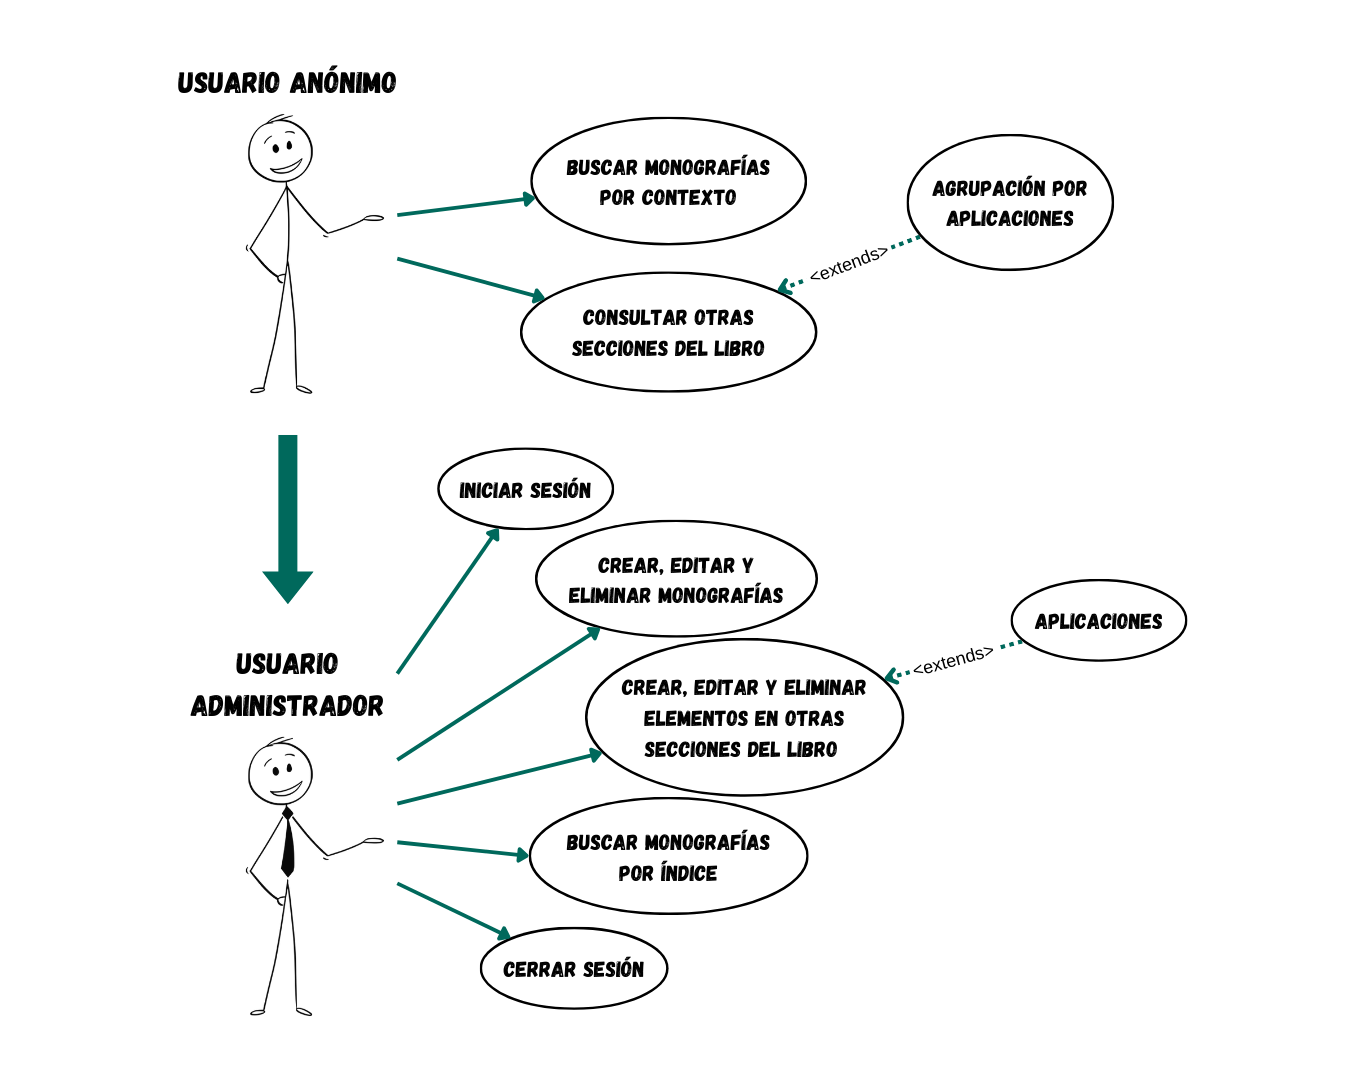
\includegraphics[width=0.9\textwidth]{Images/use-cases.png}
    \caption{Diagrama de casos de uso}
    \label{fig:use-cases}
\end{figure}




\section{Diseño de la solución}
Es posible identificar dos subproblemas principales dentro del contexto del problema anteriormente descrito mediante requerimientos. 
Estos subproblemas están interrelacionados y son fundamentales para garantizar que el sistema cumpla 
con los objetivos establecidos:

\begin{itemize}
    \item \textbf{Problema de la extracción de la información}: Este subproblema se refiere al proceso 
    de extraer, estructurar y almacenar de manera eficiente la información contenida en el libro de Tomás Roig, 
    de forma que estos datos puedan ser consumidos por un software computacional.
    \item \textbf{Problema del sistema de gestión y visualización de la información}: Una vez 
    extraída y estructurada la información, surge el desafío de diseñar e implementar un sistema que permita 
    gestionar y visualizar eficientemente los datos.
\end{itemize}

Esta sección tiene como objetivo presentar las estrategias y propuestas de diseño abstracto desarrolladas 
para abordar los subproblemas identificados anteriormente. 
Estos subproblemas, requieren soluciones específicas que garanticen tanto 
la fidelidad de los datos extraídos como su presentación efectiva a los usuarios finales.

En esta sección, se describirán los enfoques conceptuales diseñados para resolver cada 
uno de los subproblemas, teniendo en cuenta los requerimientos funcionales previamente establecidos. 
Se analizarán las características principales de cada solución, incluyendo sus componentes clave y cómo 
estos se integran para formar un sistema coherente y eficiente. Este análisis establecerá las bases 
para la implementación detallada del sistema.


\subsection{Extracción de la información}
Una solución al problema planteado debe partir de un análisis exhaustivo del corpus sobre el cual se 
realizará la extracción de información. En este sentido, tras examinar detalladamente el libro 
\textit{``Plantas medicinales, aromáticas o venenosas de Cuba''}, se identificaron una serie de observaciones 
preliminares. Estas observaciones constituyen la base para tomar decisiones informadas respecto 
a las estrategias de extracción de información que sean adecuadas y acordes con el estado del arte.

Las observaciones identificadas son las siguientes:
\begin{enumerate}
    \item La obra está dividida en dos tomos, por lo que es deseable que la solución adoptada sea 
    lo más general posible, permitiendo su aplicación efectiva en ambos tomos.
    \item Ambos tomos se encuentran en el formato: \textit{Portable Document Format} (PDF)
    \item Aunque pertenecen a la misma editorial, existen diferencias significativas 
    en cuanto a la maquetación y el diseño digital entre ambos tomos.
    \item Las monografías constituyen la sección fundamental del libro.
    \item El tomo 1 contiene las monografías de las plantas cuyos nombres inician con las letras de 
    la `A' a la `K', mientras que el tomo 2 abarca aquellas cuyas iniciales están entre la `L' y la `Z'.
    \item En las monografías se pueden identificar secciones principales que contienen cierta información 
    sobre las plantas. Estas secciones mantienen un orden fijo, aunque no siempre están 
    presentes todas en cada monografía. Las secciones identificadas son:
    \begin{itemize}
        \item Nombre con que se conoce la plantas.
        \item Nombre científico.
        \item Sinónimos.
        \item Otros nombres vulgares asociados.
        \item Hábitat y distribución geográfica.
        \item Descripción botánica.
        \item Composición química.
        \item Partes empleadas.
        \item Propiedades medicinales.
        \item Aplicaciones.
        \item Cultivo.
        \item Referencias bibliográficas.
    \end{itemize}
    \item Algunas monografías incluyen imágenes de baja calidad de las plantas, 
    acompañadas de un pie de foto que identifica el nombre de la especie.
    \item El formato de presentación del texto no es uniforme, lo que responde a decisiones editoriales y 
    de diseño. Por ejemplo, las monografías están dispuestas en una sola columna para facilitar la lectura continua, 
    mientras que otras secciones como la dedicada a la agrupación de plantas según sus aplicaciones 
    están organizadas en tres columnas para optimizar el uso del espacio al listar múltiples nombres.
\end{enumerate}

Estas características del corpus son consideradas para garantizar que la solución propuesta sea capaz de 
abordar los retos específicos que plantea la extracción de información en un contexto tan heterogéneo.

Es factible realizar la extracción del texto contenido en los documentos en formato \textit{PDF} mediante el uso 
de lenguajes de programación modernos, apoyándose en bibliotecas especializadas para la manipulación y 
el procesamiento de este tipo de archivos. No obstante, debe considerarse que el texto presenta 
características de maquetación no uniformes a lo largo de la obra, lo que podría requerir un manejo 
cuidadoso de las estructuras y formatos para asegurar una extracción precisa y completa.

En la sección \ref{section: nlp} se describe el problema general de la IE, identificándola como una 
de las tareas más comunes y relevantes en el ámbito del Procesamiento del NLP. La IE
se enfoca en identificar, estructurar y representar conocimiento relevante a partir de 
textos no estructurados o semiestructurados.

Dadas las características del corpus objeto de estudio y su estructura textual, la técnica seleccionada 
para llevar a cabo el proceso de extracción de información es la denominada \textit{template filling} abordada en la sección \ref{section: templateFilling}. 
Esta técnica permite extraer información específica mediante la identificación de patrones 
predefinidos y su mapeo en plantillas estructuradas. La elección de esta metodología 
responde a varios factores:
\begin{enumerate}
    \item La necesidad de obtener los datos en un formato estructurado que facilite su posterior uso
    en sistemas computacionales.
    \item La importancia de preservar las palabras y expresiones originales del autor 
    para garantizar una representación precisa del contenido de la obra.
    \item La adecuación de esta técnica para procesar textos con una organización semiuniforme, 
    como las monografías presentes en la obra, permitiendo capturar información clave como 
    nombres científicos, descripciones botánicas, propiedades y aplicaciones.
\end{enumerate}

Para mayor conveniencia, se optará por realizar la extracción de información del libro de manera segmentada, 
abordando cada sección de forma independiente. Este enfoque permite aplicar el proceso de \textit{template filling} 
a cada sección por separado, lo cual simplifica significativamente los algoritmos necesarios para la extracción.



\subsubsection{Template Filling en monografías}
Para la extracción de información de las monografías, se optará por un enfoque basado en reglas, 
considerando las características semiestructuradas de los datos presentes en esta sección del libro. 
El diseño de la plantilla requerirá abordar tres aspectos fundamentales: la definición 
de la estructura de la plantilla, la especificación de las reglas de interpretación 
y la documentación de casos. Sin embargo, este último punto no será desarrollado, 
dado que su utilidad sería limitada en ausencia de un enfoque basado en aprendizaje automático.

En una etapa inicial, es posible extraer la información correspondiente a cada monografía 
de manera básica. Esto implica definir una plantilla inicial que incluya los nombres de 
todas las plantas mencionadas en el libro, asociando a cada nombre el texto plano que 
representa la información respectiva. La regla de interpretación empleada en este paso se 
encargará de identificar el inicio de cada monografía, utilizando como criterio el nombre de 
la planta, que se encuentra destacado con un tamaño de fuente significativo en el texto.

A partir de esta extracción inicial, se procederá a estructurar la información de cada monografía 
basándose en su contenido. En la Figura \ref{fig:template-monograph}, se presenta la definición de la plantilla utilizada 
para este propósito, en la que se incluye el nombre de cada atributo, junto con el tipo de dato del mismo.

\begin{figure}[ht!]
    \centering
    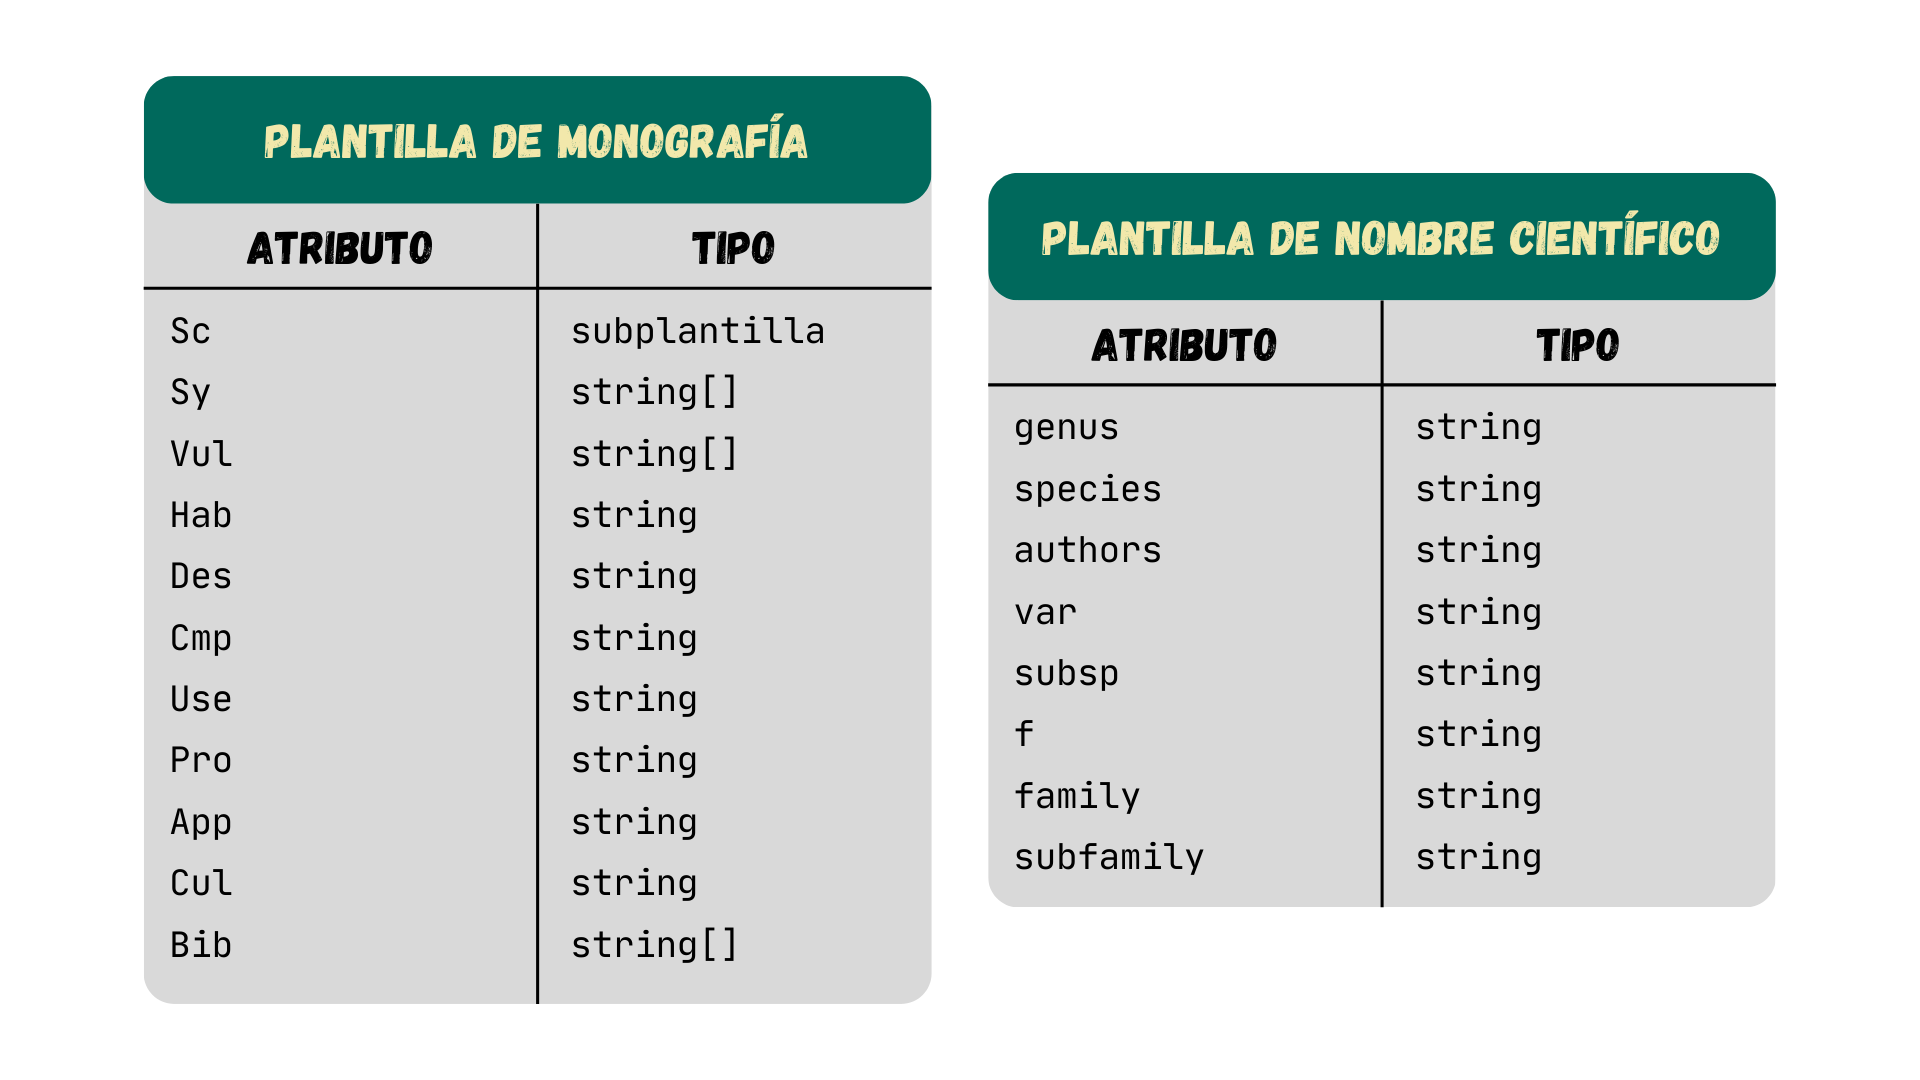
\includegraphics[width=1\textwidth]{Images/monograph-template.png}
    \caption{Plantillas de monografía y nombre científico}
    \label{fig:template-monograph}
\end{figure}

Cada atributo de la plantilla corresponde a una sección identificable dentro del contenido 
de una monografía. Por ejemplo, 
\texttt{Sc} representa el nombre científico, 
\texttt{Sy} los sinónimos,
\texttt{Vul} los nombres vulgares asociados, 
\texttt{Hab} el hábitat y distribución geográfica, 
\texttt{Des} la descripción botánica, 
\texttt{Cmp} la composición química, 
\texttt{Use} las partes empleadas, 
\texttt{Pro} las propiedades medicinales, 
\texttt{App} las aplicaciones, 
\texttt{Cul} el cultivo y 
\texttt{Bib} las referencias bibliográficas.

Como se observa en la Figura \ref{fig:template-monograph}, este diseño emplea una plantilla híbrida 
que combina características de plantillas planas y plantillas orientadas a objetos, 
permitiendo que los atributos puedan almacenar tanto datos primitivos como subplantillas, 
lo que facilita una representación más estructurada y flexible de la información.

Definamos entonces las reglas de interpretación para la plantilla de las monografías:
\begin{enumerate}
    \item Las secciones dentro de una monografía siempre aparecen en el mismo orden, y no necesariamente aparecen todas en una monografía.
    \item El nombre científico siempre aparece en la primera línea inmediatamente después del título de la monografía.
    \item Los sinónimos están precedidos por la cadena de texto \texttt{``SINÓNIMOS:''} y se encuentran separados entre sí por comas (\texttt{,}).
    \item Los otros nombres vulgares están precedidos por la cadena de texto \texttt{``OTROS NOMBRES VULGARES:''}. Los nombres correspondientes a un mismo territorio están separados por comas (\texttt{,}), mientras que los nombres entre territorios están separados por punto y coma (\texttt{;}).
    \item El texto correspondiente al hábitat y distribución está precedido por la cadena de texto \texttt{``HÁBITAT Y DISTRIBUCIÓN:''}.
    \item El texto correspondiente a la descripción botánica está precedido por la cadena de texto \texttt{``DESCRIPCIÓN BOTÁNICA:''}.
    \item El texto correspondiente a la composición química está precedido por la cadena de texto \texttt{``COMPOSICIÓN:''}.
    \item El texto correspondiente a las partes empleadas está precedido por la cadena de texto \texttt{``PARTES EMPLEADAS:''}.
    \item El texto correspondiente a las propiedades de la planta está precedido por la cadena de texto \texttt{``PROPIEDADES:''}.
    \item El texto correspondiente a las aplicaciones está precedido por la cadena de texto \texttt{``APLICACIONES:''}.
    \item El texto correspondiente al cultivo de la planta está precedido por la cadena de texto \texttt{``CULTIVO:''}.
    \item El texto correspondiente a las referencias bibliográficas está precedido por la cadena de texto \texttt{``BIBLIOGRAFÍA''}, y cada bibliografía termina en el año correspondiente a la misma.
\end{enumerate}

En cuanto a los nombres científicos, se pueden definir las siguientes reglas en función de la plantilla:
\begin{enumerate}
    \item Las partes que componen un nombre científico siempre siguen un orden específico, aunque no necesariamente todas deben estar presentes.
    \item Las primeras dos palabras corresponden al género y la especie, respectivamente.
    \item La autoridad de la planta siempre aparece inmediatamente después del género y la especie.
    \item La variedad siempre está precedida por la cadena de texto \texttt{``var.''}.
    \item La subespecie siempre está precedida por la cadena de texto \texttt{``subsp.''}.
    \item La forma siempre está precedida por la cadena de texto \texttt{``f.''}.
    \item La familia siempre está precedida por la cadena de texto \texttt{``Fam.''}.
    \item La subfamilia siempre está precedida por la cadena de texto \texttt{``Subfam.''}.
\end{enumerate}

Con la definición de estas plantillas y reglas de interpretación, se logra un diseño adecuado para 
la extracción de la información de las monografías, asegurando que los datos sean identificados y 
estructurados correctamente de acuerdo con su formato original.


\subsubsection{Template Filling en agrupación de plantas por aplicaciones}
La sección del libro que agrupa las plantas según sus aplicaciones se presenta con un diseño de 
tres columnas, optimizado para maximizar el uso del espacio disponible. En consecuencia, será 
necesario realizar una lectura ordenada que permita obtener el texto plano de toda la sección, 
a fin de aplicar la técnica de \textit{template filling}.

De manera análoga a lo realizado en la sección de las monografías, se empleará un enfoque basado 
en reglas para abordar esta sección del libro. Inicialmente, es posible identificar todas las aplicaciones 
mencionadas, bajo la regla de que los nombres de las aplicaciones aparecen completamente en mayúsculas y 
finalizan con el caracter de dos puntos (\texttt{:}), mientras que los nombres de las plantas contienen caracteres en minúsculas.
Esto nos lleva a tener una plantilla que tiene como atributos los nombres de todas las aplicaciones.

Al analizar la sección, se observa que algunas aplicaciones incluyen referencias a otras ya mencionadas, 
debido a que estas representan sinónimos o significados equivalentes. En estos casos, resulta útil que 
cada aplicación cuente con una lista de sinónimos que agrupe dichas referencias. Por lo tanto, se definirá 
una subplantilla como tipo de cada atributo en la plantilla anterior, adoptando la estructura ilustrada en 
la Figura \ref{fig:template-app}.

\begin{figure}[ht!]
    \centering
    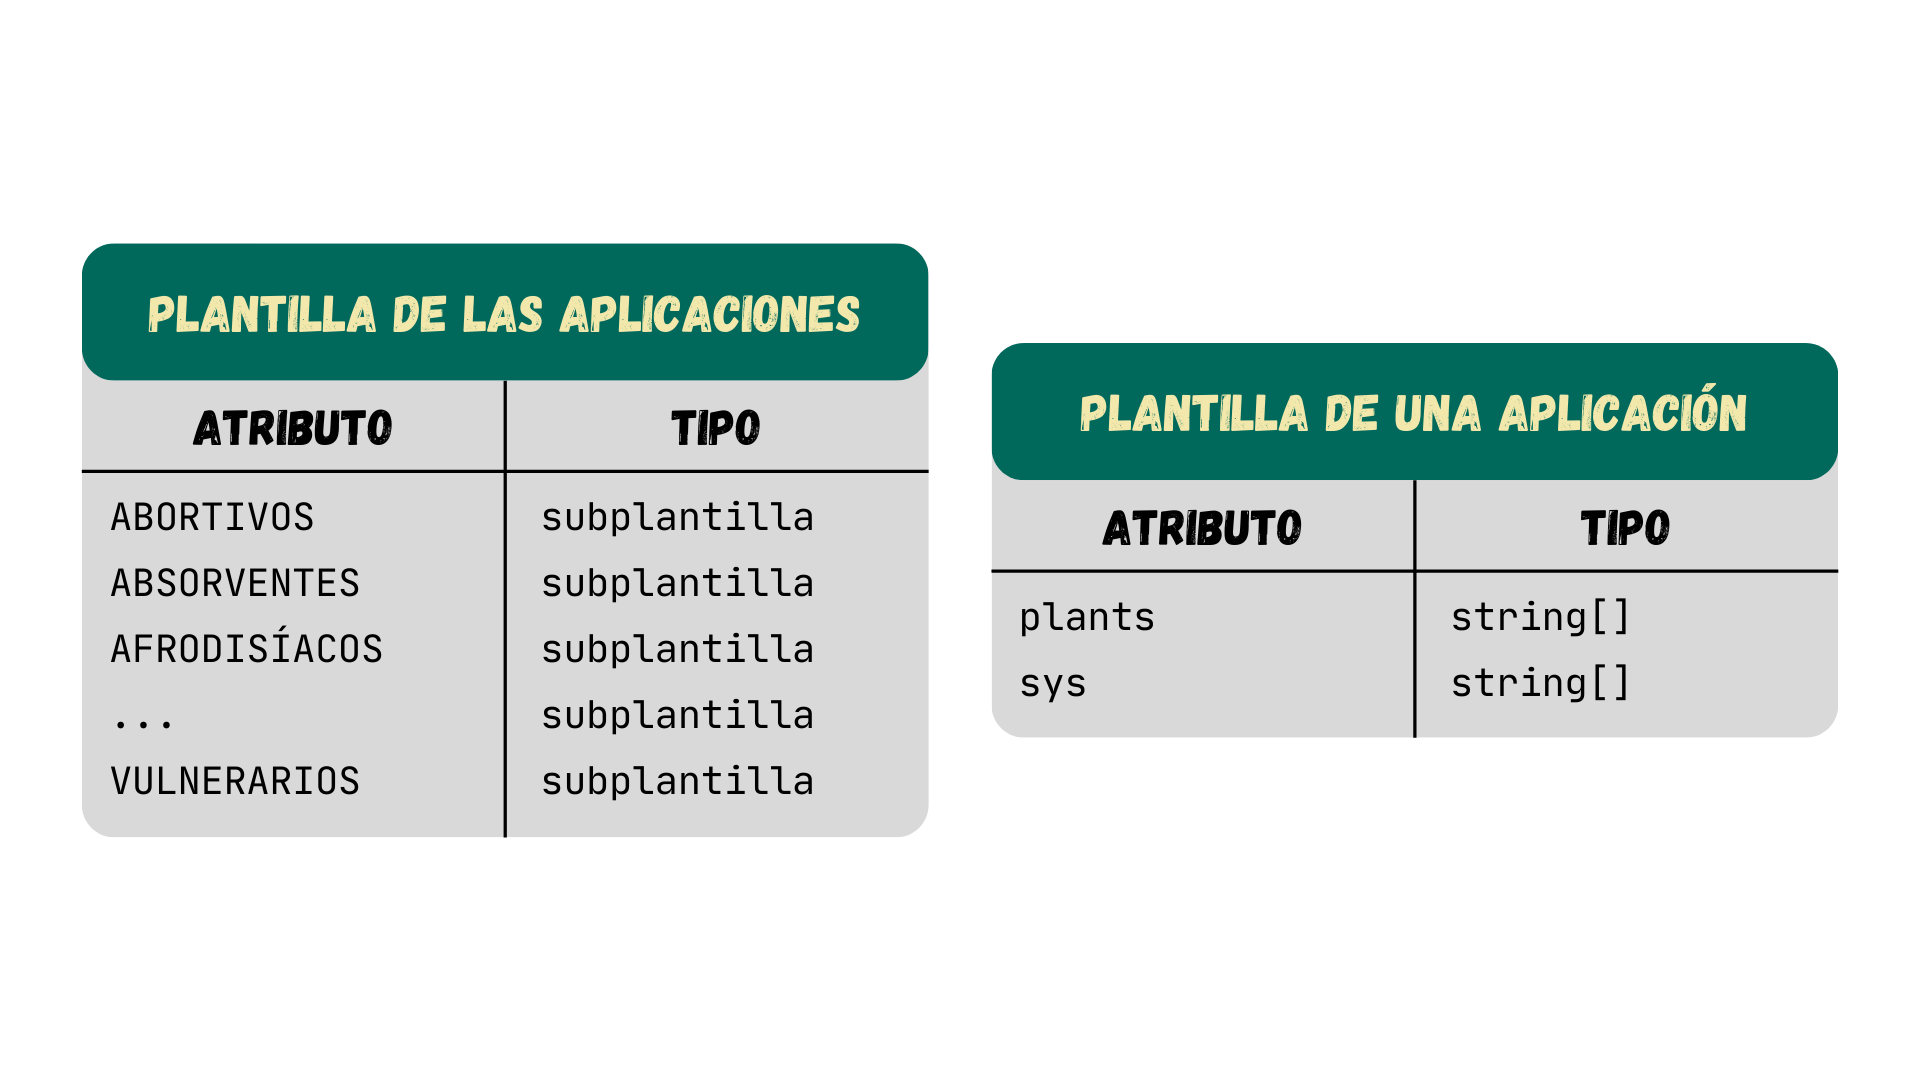
\includegraphics[width=1\textwidth]{Images/app-template.png}
    \caption{Plantillas de aplicaciones}
    \label{fig:template-app}
\end{figure}

Es posible observar que para cada aplicación tendremos una subplantilla que almacena dos listas, una con los nombres
de todas las plantas que tienen esa aplicación, y otra con los sinónimos identificados en el texto.

En base a lo anterior definimos las reglas de llenado:

\begin{enumerate}
    \item Las plantas asociadas a cada aplicación comienzan con el nombre de esta última, seguido por el caracter de dos puntos (\texttt{:}).
    \item En general, los nombres de las plantas se identifican por los saltos de línea, salvo en algunos casos excepcionales.
    \item Los casos excepcionales incluyen palabras que no caben en una misma línea, las cuales se indican mediante un guion (\texttt{-}), señalando que el nombre continúa en la siguiente línea.
    \item Algunas aplicaciones presentan, justo a continuación de su nombre, el nombre de otra aplicación entre paréntesis, lo que indica que heredan las plantas asociadas a esta última.
    \item Las referencias a otras aplicaciones se identifican por la cadena de caracteres \texttt{``Véase''}, seguida del nombre de la aplicación correspondiente.
\end{enumerate}




\subsection{Sistema de gestión y visualización}
El diseño de un sistema web eficiente y escalable requiere la separación clara entre el frontend y el backend, 
siguiendo los principios de modularidad y responsabilidad única. El frontend se ocupa de la presentación y 
experiencia del usuario, mientras que el backend se encarga de procesar la lógica del negocio, gestionar la 
persistencia de datos y exponer interfaces (APIs) para interactuar con el sistema. Este enfoque asegura que 
cada componente pueda desarrollarse, mantenerse y escalarse de manera independiente.

En el caso del backend, se empleará una arquitectura por capas que permita una separación clara de responsabilidades. 
Esta arquitectura incluirá las siguientes capas principales:

\begin{enumerate}
    \item \textbf{Capa de datos}: Responsable de modelar las entidades del dominio.
    \item \textbf{Capa de acceso a datos}: Proveerá métodos especializados para interactuar con la base de datos, 
    aislando las operaciones sobre la misma de la lógica de negocio.
    \item \textbf{Capa de servicios}: Implementará la lógica del negocio y las reglas del sistema, ofreciendo 
    funcionalidades como servicios que serán consumidos posteriormente.
\end{enumerate}

Estas capas estarán integradas en un proyecto principal de backend, cuya función será consumir los servicios para exponer una serie de APIs 
que sirvan como puente entre los frontends y la lógica del sistema. Este diseño por capas garantiza mantenibilidad, 
escalabilidad y reutilización del código.

Debido a los requerimientos del sistema, se necesitarán dos módulos principales: un módulo de administración y 
un módulo orientado al cliente final de internet. Cada uno de estos módulos contará con un proyecto independiente 
de frontend para cubrir las necesidades específicas de cada tipo de usuario. Este enfoque asegura que ambos 
módulos sean autónomos en su desarrollo y despliegue, al tiempo que se preserva la consistencia general del sistema.

Para optimizar el uso de recursos y evitar redundancias, las capas de datos, acceso a datos y servicios del backend 
serán compartidas entre los módulos. Esto significa que, aunque se desarrollen dos proyectos de web API 
(uno para el módulo de administración y otro para el cliente final), ambos consumirán las mismas capas internas de 
lógica y acceso a datos. De esta manera, se centraliza la lógica común en un solo lugar, promoviendo la 
reutilización del código, simplificando el mantenimiento y facilitando la escalabilidad del sistema ante posibles 
cambios o nuevas funcionalidades en el futuro. En la Figura \ref{fig:architecture} se ilustra la arquitectura explicada del sistema.

\begin{figure}[ht!]
    \centering
    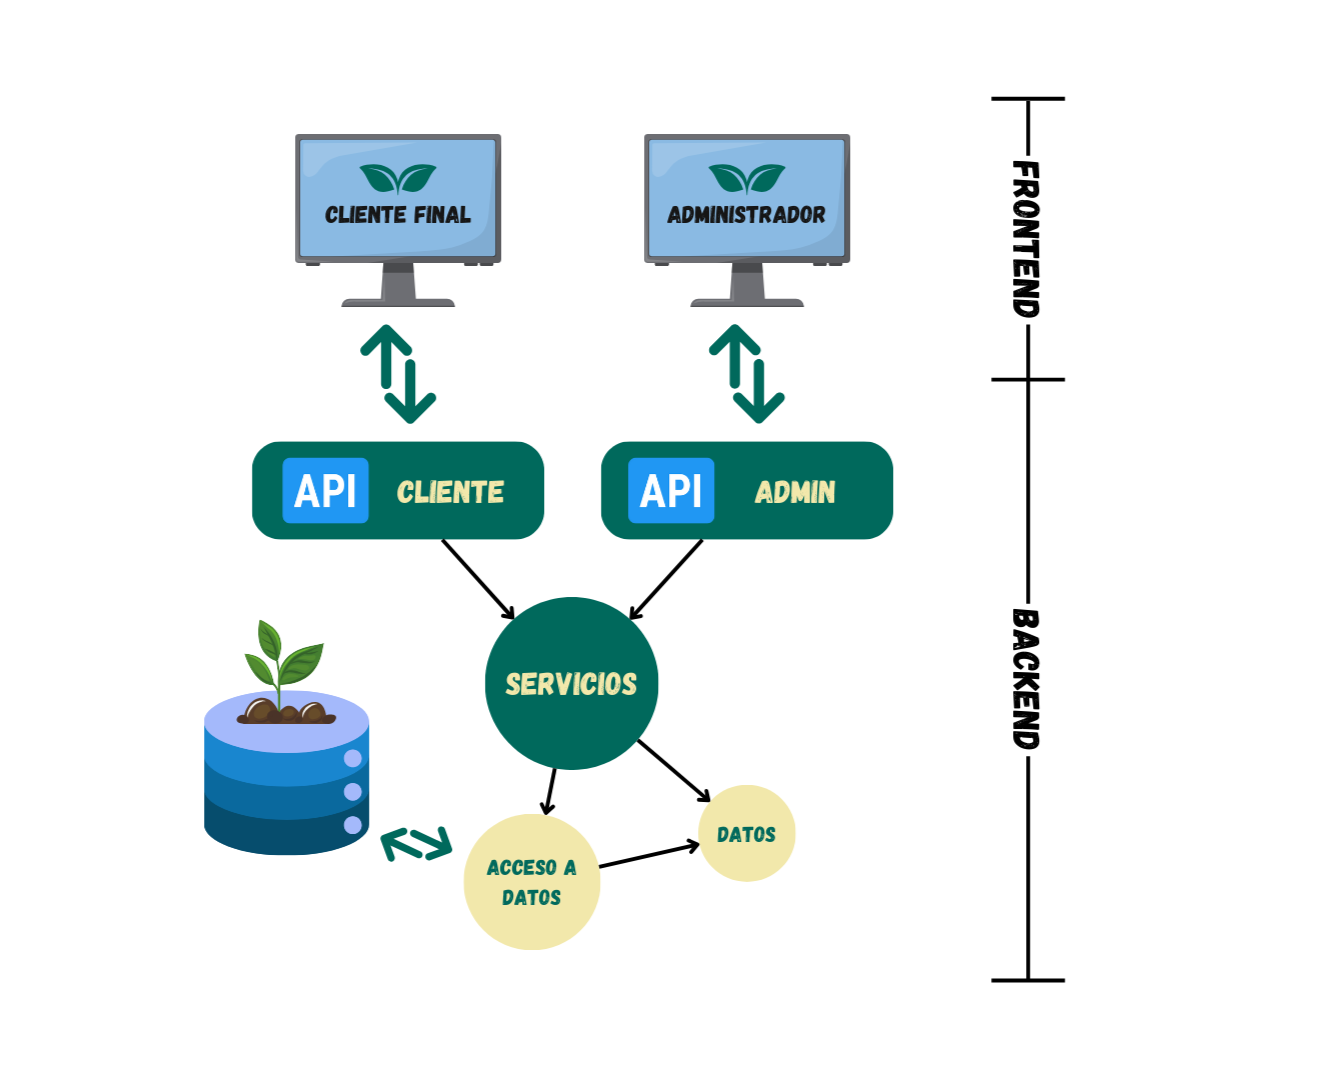
\includegraphics[width=0.9\textwidth]{Images/architecture.png}
    \caption{Arquitectura del sistema}
    \label{fig:architecture}
\end{figure}

\subsubsection{El modelo de datos}
El modelo de datos proporciona la estructura necesaria para almacenar, gestionar y acceder de manera eficiente a la información. 
Basado en las entidades fundamentales del dominio, el modelo representa los elementos clave que se gestionarán a lo largo de su 
ciclo de vida, estableciendo relaciones entre ellos. Es esencial que el diseño de estas relaciones esté bien estructurado, 
alineado con los requerimientos funcionales y las características del sistema, para garantizar la alta integridad y disponibilidad 
de los datos, así como para facilitar las consultas y optimizar el rendimiento del sistema.

Los principales componentes del modelo de datos son:

\begin{enumerate} 
    \item \textbf{Entidades del dominio}: Son los objetos principales con los que interactuarán los usuarios y el sistema. 
    En nuestro caso, estas entidades incluyen elementos como plantas, términos, aplicaciones y usuarios. Cada entidad está representada 
    por una tabla en la base de datos, y sus atributos corresponden a las columnas de dichas tablas.
    \item \textbf{Relaciones entre entidades}: Las entidades no operan de manera aislada, sino que están interconectadas entre sí. Las relaciones 
    entre las entidades pueden ser de uno a uno, uno a muchos o muchos a muchos, y deben estar modeladas adecuadamente en el esquema de la 
    base de datos. Estas relaciones permiten que los datos sean accesibles y actualizados de manera coherente en todo el sistema.
    \item \textbf{Normalización y optimización}: Para garantizar la eficiencia en el acceso y la integridad de los datos, se llevará a cabo un 
    proceso de normalización. La normalización busca reducir la redundancia de los datos y mejorar la consistencia de las relaciones. Esto significa 
    que cada tipo de información debe estar en su lugar adecuado, sin duplicar datos innecesarios.
    Además, se implementarán índices y claves foráneas para optimizar las consultas y mantener la integridad referencial.
    \item \textbf{Persistencia de datos}: El modelo de datos se implementará utilizando una base de datos relacional, que proporcionará las herramientas 
    necesarias para almacenar, consultar y actualizar la información de manera eficiente. 
    La capa de acceso a datos se encargará de interactuar con la base de datos y ofrecer las funcionalidades necesarias para las operaciones CRUD (Crear, Leer, Actualizar, Eliminar).
\end{enumerate}

El modelo de datos será la base sobre la cual se construirán los servicios y las APIs del sistema. Cada operación o servicio del backend interactuará con la base de datos a través 
de las capas de acceso a datos y servicios, garantizando que las transacciones sean consistentes y eficaces.

El modelo de relaciones está basado en un enfoque de muchos a muchos entre las entidades Planta y Término (a través de PlantTerm), así como entre Planta y Aplicación (a través de PlantApp). 
Estas relaciones intermedias permiten flexibilidad en el sistema, permitiendo que cada planta esté asociada a múltiples términos y aplicaciones y viceversa, y de esta forma mantener la integridad 
referencial y evitar problemas de redundancia. 

En el caso de la entidad Usuario, no se encuentra interrelacionada directamente con las demás entidades, siendo completamente autónoma, lo que simplifica su manejo y permite 
que los usuarios interactúen con el sistema sin necesidad de relaciones directas con las demás entidades del dominio.

Para facilitar la comprensión de la estructura de la base de datos, el diagrama de la Figura \ref{fig:merx} ilustra el modelo Entidad-Relación-Extendido (MERX) del sistema, que refleja las entidades principales y sus relaciones clave.

\begin{figure}[ht!]
    \centering
    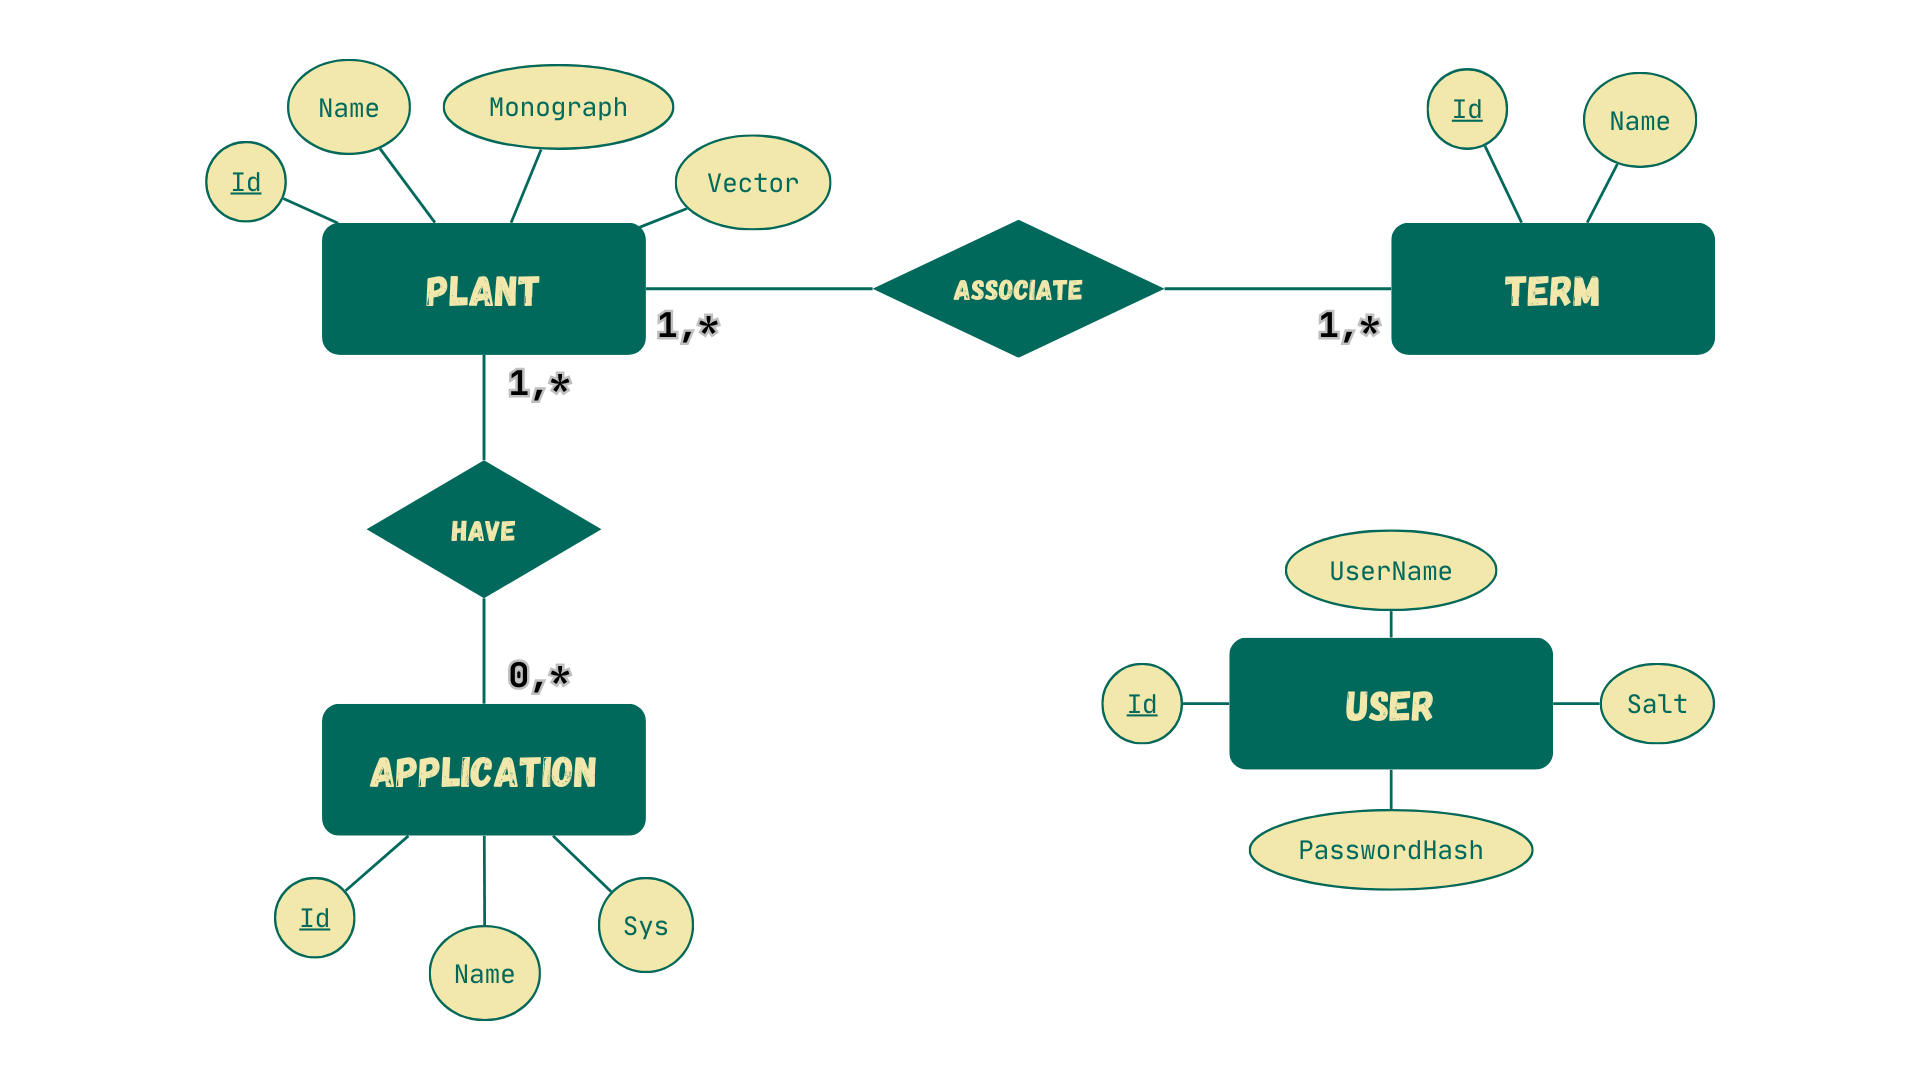
\includegraphics[width=0.9\textwidth]{Images/merx.png}
    \caption{MERX}
    \label{fig:merx}
\end{figure}

\chapter{Implementación y experimentación}\label{chapter:implementation}
En el presente capítulo se presentan los elementos prácticos que han sido empleados para 
materializar la solución conceptualizada en el diseño previo. El objetivo principal es 
detallar cómo se implementaron las diversas tecnologías, metodologías y herramientas 
seleccionadas para construir un sistema funcional que cumpla con los 
requisitos establecidos y los objetivos trazados.

Se expondrá en primer lugar la identidad del sitio web, destacando las decisiones relacionadas 
con su diseño visual y los elementos que refuerzan su alineación con los valores de marca del 
Jardín Botánico Nacional de Cuba. Posteriormente, se describirán de manera estructurada los 
procesos técnicos y las decisiones tomadas durante la implementación, haciendo énfasis en 
aspectos clave como la selección de tecnologías, la organización del código y las estrategias 
empleadas para integrar y probar los componentes del sistema.

Además, se discutirán los retos encontrados durante esta etapa y las soluciones 
adoptadas para superarlos, asegurando que el producto final sea técnicamente robusto 
y alineado con las necesidades del proyecto.

Se explicarán por separado las soluciones propuestas para las dos problemáticas 
abordadas en el capítulo anterior. Este enfoque se adopta porque cada problemática puede 
considerarse un problema independiente, lo que facilita una comprensión más clara y detallada 
de la solución final.

Adicionalmente, se incluyen las primeras pruebas experimentales realizadas con la solución implementada, 
con el fin de evaluar su desempeño y validar que los resultados obtenidos cumplen con las 
expectativas definidas en las fases iniciales. Estos experimentos no solo verifican el cumplimiento 
funcional, sino que también permiten identificar posibles áreas de mejora o ajuste, 
garantizando que el sistema sea escalable y adaptable a futuros requerimientos.



\section{Identidad del sitio}
El sistema desarrollado como resultado de este trabajo ha sido nombrado\newline \textbf{BotaniQ}, un nombre 
que refleja de manera directa su propósito y esencia. La elección de este nombre surge de la 
combinación de dos elementos clave: la palabra \textit{``botánica''}, que alude al estudio de las plantas, 
y la letra \textit{``Q''}, que hace referencia a \textit{``query''} (significa consulta en inglés),
resaltando su función principal como una herramienta para la consulta y gestión de información sobre plantas medicinales. 
Este nombre busca transmitir simplicidad, profesionalismo y un enfoque claro en la temática del 
proyecto, a la vez que facilita su identificación y asociación con su objetivo principal.
En la Figura \ref{fig:botaniq} se muestra el logotipo de BotaniQ.

\begin{figure}[ht!]
    \centering
    
\includegraphics[width=0.25\textwidth]{Images/botaniq.png}
    \caption{Logotipo de BotaniQ}
    \label{fig:botaniq}
\end{figure}

Las interfaces de BotaniQ están diseñadas para reflejar y reforzar un valor de marca que pueda 
asociarse directamente con el Jardín Botánico Nacional de Cuba. Para lograr este propósito, 
se ha adoptado una paleta cromática basada en los colores primario y secundario presentes en 
el logotipo de dicha institución, asegurando así una identidad visual coherente y representativa.
La paleta de colores se muestra en la Figura \ref{fig:palette}.

\begin{figure}[ht!]
    \centering
    
\includegraphics[width=1\textwidth]{Images/palette.png}
    \caption{Paleta de colores}
    \label{fig:palette}
\end{figure}

Para garantizar que el diseño del sitio web BotaniQ transmita una identidad visual acorde a su 
propósito, se seleccionaron fuentes tipográficas que equilibran profesionalismo, claridad y frescura, 
alineadas con la temática botánica y científica del proyecto. Estos estilos son accesibles
libre de costo desde el sitio: \href{https://fonts.google.com/}{Google Fonts}. 
Una muestra de estos estilos se puede apreciar en la Figura \ref{fig:fonts}.

\begin{itemize}
    \item Estilo primario: \texttt{Montserrat Alternates}
    \item Estilo secundario: \texttt{Quicksand}
    \item Estilo complementario: \texttt{Sniglet}
\end{itemize}


\begin{figure}[ht!]
    \centering
    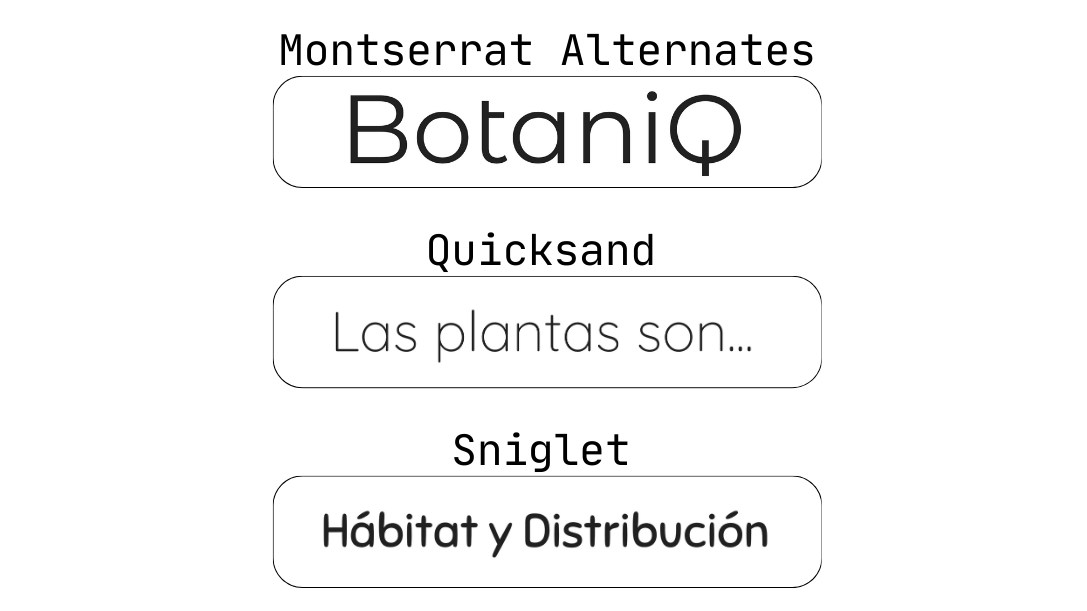
\includegraphics[width=1\textwidth]{Images/fonts.png}
    \caption{Fuentes tipográficas}
    \label{fig:fonts}
\end{figure}



\section{Solución al problema de Extracción de información}
Para implementar esta solución, se seleccionó 
\textbf{Python}\footnote{Visitar en \url{https://www.python.org}} como lenguaje de programación 
debido a su versatilidad, facilidad de uso y la sólida comunidad que lo respalda, ofreciendo 
una amplia variedad de bibliotecas para diversas tareas. Python es un lenguaje de 
programación interpretado, de alto nivel y multiparadigma, que permite trabajar con estilos 
como la programación orientada a objetos, funcional y procedimental. Su diseño enfatiza la 
legibilidad del código, lo que facilita el desarrollo y mantenimiento de proyectos.

En este contexto, se eligieron las bibliotecas 
\texttt{PyMuPDF}\footnote{Visitar en \url{https://pypi.org/project/PyMuPDF/}} y 
\texttt{pdfplumber}\footnote{Visitar en \url{https://pypi.org/project/pdfplumber/}} para 
abordar la lectura de los documentos en formato \textit{PDF}. La biblioteca \texttt{PyMuPDF} 
fue escogida principalmente por su extensa documentación y su eficacia en la extracción de 
texto de manera uniforme, lo que resulta fundamental para garantizar una base inicial 
consistente de los datos extraídos. Por otro lado, \texttt{pdfplumber} se seleccionó por las 
ventajas que ofrece en términos de manejo del diseño del documento, particularmente su 
capacidad para identificar y encuadrar bloques de texto.

La información extraída será almacenada en un archivo en formato \textit{JSON}. Este formato 
es ampliamente utilizado en la actualidad debido a su capacidad para representar datos de 
manera estructurada y su gran adaptabilidad en los sistemas computacionales modernos. 
\textit{JSON} es un formato ligero y de fácil lectura tanto para humanos como para máquinas, 
lo que lo convierte en una opción ideal para la interoperabilidad entre diferentes sistemas 
y plataformas, especialmente en aplicaciones web y servicios API.

Tal como se expuso en el capítulo anterior, se adoptará un enfoque basado en \textit{template filling} 
para estructurar la información extraída. Las plantillas se implementarán como diccionarios de Python, 
una estructura de datos que permite almacenar información en pares clave-valor de forma eficiente. 
Los diccionarios son fundamentales para garantizar una representación coherente y ordenada de los datos, 
facilitando su posterior transformación al formato \textit{JSON}.

Para la implementación del flujo de llenado de plantillas, se adoptó un estilo de programación imperativa. 
El llenado de las plantillas 
se realizó de manera jerárquica, progresando desde los niveles más generales hacia los más específicos. 
En otras palabras, primero se completaron los atributos simples de la plantilla principal, y posteriormente 
se procedió al llenado de los atributos que corresponden a subplantillas.

Este enfoque permite encapsular las reglas de llenado de las subplantillas en algoritmos independientes, 
lo que no solo mejora la modularidad del código, sino que también facilita la comprensión y el mantenimiento 
del flujo de trabajo. Al trabajar con subplantillas de manera autónoma, se asegura que cada componente de la 
plantilla sea manejado de forma eficiente y aislada, reduciendo la complejidad del sistema general y permitiendo 
futuros ajustes o ampliaciones de manera más sencilla.

Durante el desarrollo del algoritmo para la extracción de las monografías, surgieron ciertos problemas que 
requirieron ser resueltos sobre la marcha. Estas dificultades se debieron, en algunos casos, a excepciones 
en las reglas de llenado previamente definidas, ya sea por errores tipográficos en el texto original o por 
inconsistencias durante el proceso de extracción del contenido del libro. Entre los problemas identificados 
se encuentran los siguientes:

\begin{itemize}
    \item Secciones en las que no se detectó la palabra clave que determina su inicio fueron insertadas 
    erróneamente como una continuación de la sección previamente identificada.
    \item Duplicación de nombres de monografías idénticos, lo que generaba conflictos al intentar 
    utilizarlos como claves en los atributos de la plantilla.
    \item Inclusión de pies de página de las imágenes dentro del texto extraído.
    \item Inclusión de números de página entre el texto.
    \item Fragmentación de palabras en el texto debido al uso de guiones (\texttt{-}) cuando estas no 
    cabían en la línea del texto original, lo que afectaba la integridad del texto plano extraído.
\end{itemize}

La solución a estos problemas no fue particularmente compleja de identificar. Algunos casos, debido a su 
naturaleza limitada y a la falta de un patrón recurrente en el texto, fueron resueltos de forma directa 
y específica mediante soluciones personalizadas adaptadas a cada caso puntual.

Al finalizar el algoritmo de extracción, cada atributo que almacena una cadena de texto queda representado 
en un formato plano. Esto significa que no se preservan las separaciones de párrafos, siendo el contenido 
una simple secuencia de oraciones concatenadas. Además, en ocasiones donde el texto original contiene 
listas de elementos, estas se presentan como elementos continuos separados únicamente por espacios. 
Este tipo de formato puede dificultar la lectura y la interpretación del contenido, lo que hace 
necesario estructurarlo de manera más clara para mejorar su comprensión. Incluso una medida sencilla, 
como la inclusión de saltos de línea (\verb|\n|), puede contribuir significativamente a mejorar la legibilidad.

Para abordar este problema, se aprovecha el poder de los modelos de lenguaje para interpretar y 
generar texto de manera coherente. En este caso, se utilizó el modelo \texttt{gemini-1.5-flash} de
\textbf{Gemini}\footnote{Visitar a través de Google AI Studio en \url{https://aistudio.google.com/}}, desarrollado por Google, 
cuya elección se fundamenta en la disponibilidad de una API gratuita y su integración sencilla con lenguajes 
como Python para tareas automatizadas. Este modelo ha demostrado excelentes resultados en procesos de 
procesamiento y generación de texto. Para garantizar que el texto resultante cumpla con los requisitos esperados, 
se aplicaron técnicas de ingeniería de prompts diseñadas para guiar al modelo hacia la generación de resultados 
precisos y adecuados.

El resultado final es una plantilla completa, organizada y bien estructurada, con datos listos para ser leídos 
e interpretados de manera eficiente. Esta transformación mejora la presentación visual del contenido  
y optimiza su utilidad en contextos prácticos.

A continuación, se procedió a extraer la información correspondiente a la agrupación de plantas según sus aplicaciones. 
Similar al caso anterior, se presentaron algunos inconvenientes debido a inconsistencias en las reglas definidas 
durante el diseño de la solución o a limitaciones inherentes a la biblioteca utilizada para la extracción de texto. 
Entre los problemas identificados se encuentran:
 
\begin{itemize}
    \item En ciertos casos puntuales, nombres de plantas que continúan en la siguiente línea no fueron 
    detectados correctamente. Esto ocurrió porque, al no estar separados por un guion (\texttt{-}), 
    no se considera un corte de palabra, y la palabra en la línea siguiente comienza con mayúscula, 
    lo que impide la asociación automática.
    \item En un caso específico, un nombre de aplicación no fue identificado en su posición correspondiente, 
    lo que resultó en que su contenido fuera erróneamente incluido dentro de la aplicación anterior.
\end{itemize}

Dado que estos problemas son casos excepcionales y no recurrentes, se abordaron mediante correcciones 
directas en el código implementado.

El resultado final es una plantilla estructurada y completamente llena, representada en formato \textit{JSON}, 
que está lista para ser utilizada en otros entornos computacionales. 




\section{Solución al problema del Sistema de gestión y visualización: BotaniQ}
En el desarrollo de BotaniQ, se emplearon tecnologías modernas y ampliamente utilizadas en la industria 
para garantizar un sistema robusto, eficiente y escalable. Estas herramientas fueron seleccionadas 
cuidadosamente para abordar los requerimientos específicos del proyecto, permitiendo una implementación 
organizada y una experiencia de usuario óptima.

Para el frontend, se utilizó 
\textbf{React} \footnote{Visitar en \url{https://react.dev}}
en combinación con 
\textbf{TypeScript}\footnote{Visitar en \url{https://www.typescriptlang.org}}. 
React es una biblioteca de JavaScript enfocada en la creación de interfaces de usuario dinámicas y reactivas, estructuradas en componentes 
modulares que facilitan el desarrollo y la reutilización de elementos visuales. TypeScript, al ser un 
superconjunto tipado de JavaScript, aporta seguridad al proceso de desarrollo, permitiendo detectar 
errores antes de la ejecución y promoviendo un código más estructurado, lo cual es esencial en un 
proyecto de esta magnitud. Esta combinación mejora la experiencia del usuario final con una 
interfaz intuitiva, y facilita el mantenimiento y la escalabilidad del sistema.

En el backend, se optó por 
\textbf{ASP.NET Core}\footnote{Visitar en \url{https://dotnet.microsoft.com/en-us/apps/aspnet}}
como marco de desarrollo, una plataforma de código abierto diseñada para construir aplicaciones modernas 
de alto rendimiento. Este framework permite desarrollar servicios web estructurados que manejan eficientemente la lógica 
del negocio y el acceso a datos. 
La implementación del backend se organizó en capas previamente definidas: la capa de datos, la capa de acceso a datos y 
la capa de servicios, cada una desarrollada como una biblioteca dinámica (DLL) utilizando
\textbf{C\#}\footnote{Visitar en \url{https://dotnet.microsoft.com/en-us/languages/csharp}}.

La información se gestiona mediante una base de datos 
\textbf{PostgreSQL}\footnote{Visitar en \url{https://www.postgresql.org}},
un sistema de gestión de bases de datos relacional reconocido por su rendimiento y capacidad para manejar datos 
estructurados. A pesar de su naturaleza relacional, PostgreSQL ofrece características similares a las bases de datos NoSQL, 
como la capacidad de almacenar datos en formato JSON. Esta flexibilidad nos permite almacenar las monografías de plantas de 
manera eficiente, asegurando que, a pesar de que algunas secciones puedan estar vacías, todas las monografías sigan el mismo 
esquema gracias a la técnica de template filling. El backend es responsable de procesar las solicitudes, interactuar con 
PostgreSQL a través de la capa de acceso a datos y exponer los datos mediante servicios web que pueden ser consumidos por el frontend.

Estas tecnologías trabajan de forma integrada para garantizar 
un flujo de datos coherente y confiable entre el cliente y el servidor, asegurando que los usuarios de 
BotaniQ puedan acceder a la información de manera rápida y eficiente. Estas herramientas modernas y 
probadas en entornos de producción aseguran que el sistema sea robusto, mantenible y esté preparado para 
futuros requerimientos.

Esta estructura tecnológica se ilustra en la Figura \ref{fig:techs}, proporcionando una visión 
clara de cómo se integran los diferentes componentes del sistema.

\begin{figure}[ht!]
    \centering
    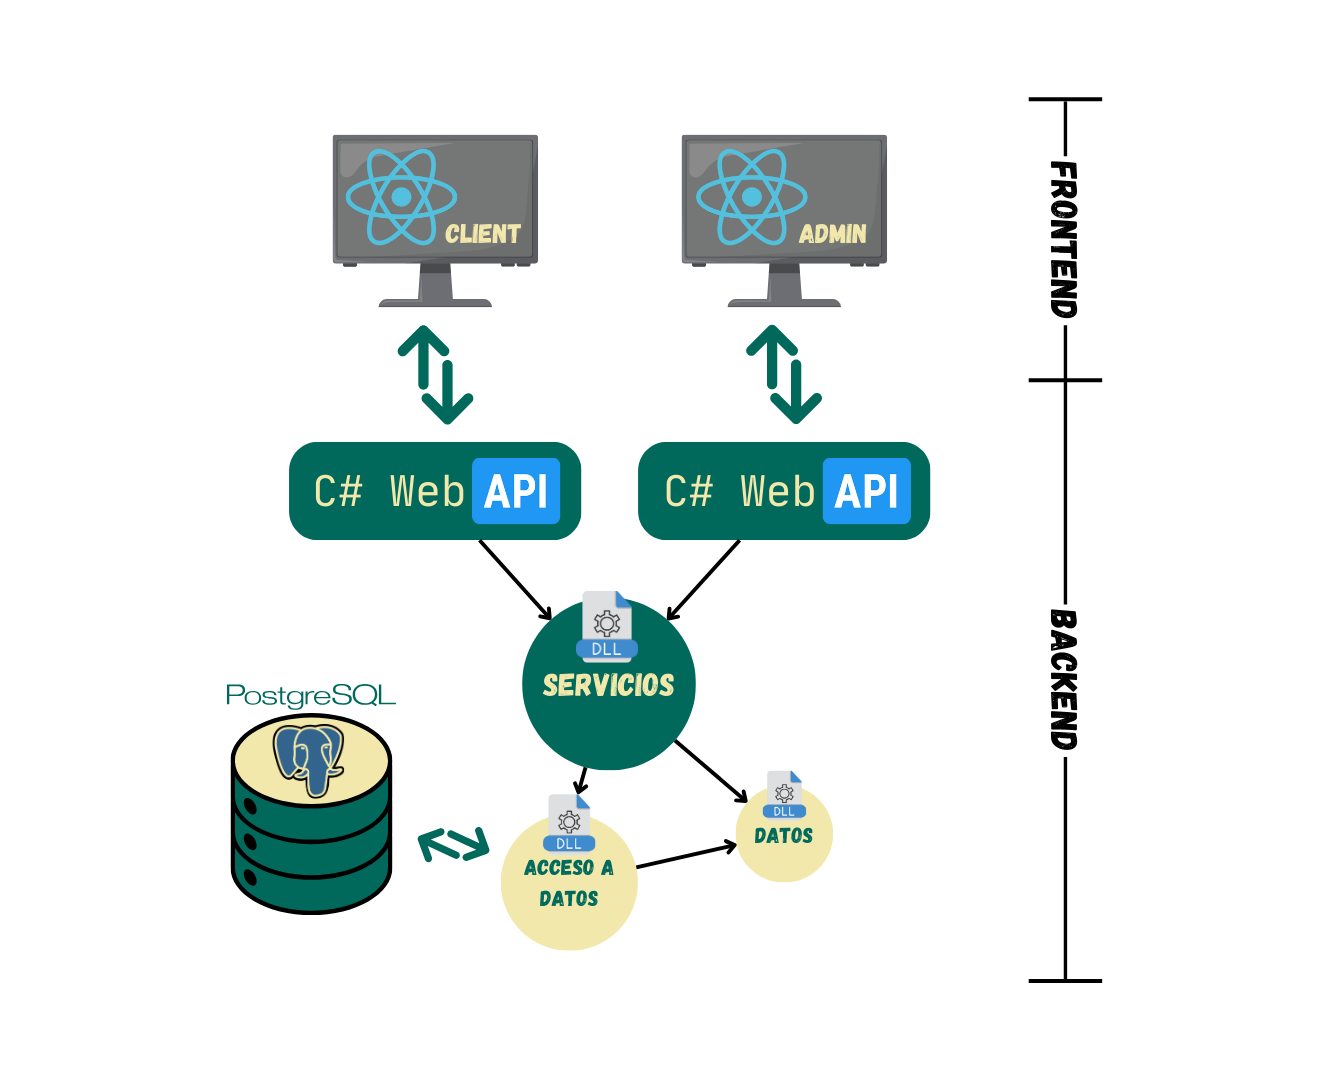
\includegraphics[width=0.9\textwidth]{Images/techs.png}
    \caption{Estructura tecnológica del sistema}
    \label{fig:techs}
\end{figure}

En ambos proyectos de frontend de BotaniQ, el desarrollo se realizó siguiendo el diseño de identidad del sitio, 
que se basa en ofrecer una experiencia visual coherente y profesional que refleje la marca asociada al 
Jardín Botánico Nacional de Cuba. A lo largo del proceso de implementación, se prestó especial atención a la 
adaptabilidad de la interfaz, asegurando que el sitio fuera completamente responsivo y brindara una experiencia 
de usuario óptima en diversos dispositivos, desde computadoras de escritorio hasta teléfonos móviles y tabletas.

Para lograr esta adaptabilidad, se utilizó 
\textbf{Tailwind CSS}\footnote{Visitar en \url{https://tailwindcss.com}},
un framework de CSS altamente flexible y eficiente que permite una personalización precisa y una creación de 
interfaces de usuario rápida y efectiva. Con Tailwind, fue posible aplicar un enfoque de diseño móvil primero, 
garantizando que la interfaz respondiera de manera eficiente a las diferentes resoluciones de pantalla sin 
perder la coherencia en su estructura visual. Además, el uso de clases utilitarias de Tailwind facilitó el 
diseño modular, lo que mejoró la mantenibilidad y escalabilidad del sistema.

Adicionalmente, se implementó 
\textbf{Flowbite}\footnote{Visitar en \url{https://flowbite.com}},
una biblioteca de componentes basada en Tailwind CSS, para acelerar el desarrollo y asegurar una interfaz de 
usuario consistente. Flowbite proporcionó una serie de componentes preconstruidos y personalizables, como 
botones, formularios y modales, lo que permitió integrar elementos interactivos con facilidad y sin necesidad 
de construir cada componente desde cero. Gracias a la combinación de Tailwind y Flowbite, se logró una 
interfaz visualmente atractiva, funcional y alineada con los principios de diseño del sitio.

Por otro lado, en el desarrollo del backend de BotaniQ, se implementaron las APIs necesarias para exponer 
los servicios que permiten la interacción entre el frontend y la base de datos. Estas APIs fueron diseñadas 
cuidadosamente para garantizar que solo se expusieran los servicios relevantes a cada uno de los dos proyectos 
de Web API, lo que contribuye a una arquitectura más organizada y segura, restringiendo el acceso a datos innecesarios.

Para la interacción con la base de datos, se utilizó 
Entity Framework Core\footnote{Visitar en \url{https://www.nuget.org/packages/EntityFramework}} 
como Object-Relational Mapper (ORM, por sus siglas en inglés),
bajo un enfoque \textit{``Code First''}, lo que permitió definir las entidades de la base de datos directamente 
en el código. Este enfoque simplificó el proceso de creación y mantenimiento del esquema de la base de datos, 
ya que las clases de C\# fueron las que definieron la estructura de las tablas y sus relaciones. Gracias a este ORM, 
se facilitó la gestión de las entidades y la realización de consultas, permitiendo que el acceso a los datos fuera 
más eficiente y seguro.

En cuanto a la base de datos, se realizó una población inicial de la misma utilizando la información extraída del 
libro de plantas medicinales. Esta operación se ejecuta la primera vez que se inicia la Web API del administrador, 
permitiendo que los datos extraídos de manera estructurada sean cargados en la base de datos de manera automática. 
Esto asegura que la base de datos esté correctamente inicializada y preparada para su uso desde el inicio.

Una característica fundamental del sistema es la capacidad de realizar búsquedas por contexto. Este mecanismo permitirá 
que el usuario pueda obtener resultados más relevantes y precisos basados en el contexto de su consulta, mejorando 
la experiencia de búsqueda y garantizando que los datos obtenidos sean los más apropiados para el usuario en cada situación. 
Este aspecto será detallado con más profundidad a continuación, pues constituye una de las funcionalidades clave incluidas en BotaniQ.


\subsection{La búsqueda por contexto}
La implementación de este mecanismo de búsqueda se lleva a cabo a través de varios componentes interconectados que incluyen controladores, 
servicios y acceso a la base de datos.

El Controlador de Consulta actúa como el punto de entrada para las solicitudes HTTP. En este caso, se encarga de gestionar las consultas de 
búsqueda que los usuarios envían a través de la API. El controlador no realiza el procesamiento de la búsqueda directamente, sino que delega 
esta tarea al servicio de búsqueda. Una vez que la consulta es recibida por el controlador, el Servicio de Búsqueda de Plantas es el responsable 
de procesarla. Este servicio contiene la lógica necesaria para analizar la consulta y calcular qué plantas de la base de datos son relevantes 
para los términos de búsqueda proporcionados.

El primer paso en el procesamiento de la consulta fue la tokenización. La entrada de texto se descompuso en unidades más pequeñas llamadas "tokens", 
que suelen ser palabras individuales o secuencias de caracteres. Durante este proceso, también se eliminaron las palabras vacías o "stop words", que 
no aportan valor semántico a la consulta. Estas palabras son descartadas para asegurar que el análisis se concentre en los términos relevantes.

Después de procesar y analizar los términos de la consulta, el siguiente paso fue buscar en la base de datos para encontrar registros 
que coincidan con estos términos. Dependiendo del diseño de la base de datos, esta búsqueda puede involucrar diferentes técnicas, tales como búsqueda 
exacta o búsqueda aproximada basada en la similitud de palabras.

En este contexto, se emplean diversos métodos, como la búsqueda exacta por término, la búsqueda basada en la distancia de Levenshtein y la búsqueda por trigramas.

\subsubsection*{1. Búsqueda Exacta por Término}

La búsqueda exacta fue el enfoque más sencillo y directo, en el que se busca una coincidencia exacta entre los términos de la consulta y los términos almacenados en 
la base de datos. Este tipo de búsqueda es muy eficaz cuando los términos introducidos por el usuario coinciden exactamente con los términos en la base de datos. 
Para asegurar que la búsqueda no se viera afectada por diferencias en tildes, se utilizó la función \texttt{unaccent} propia de PostgreSQL, que permite ignorar estas variaciones. 
De esta forma, las palabras ``planta'' y ``plántá'' son tratadas como equivalentes.

Sin embargo, este enfoque tiene limitaciones, ya que no es capaz de manejar errores tipográficos o variaciones menores en la escritura de los términos de búsqueda. 
En estos casos, el sistema recurre a métodos adicionales.

\subsubsection*{2. Búsqueda por Levenshtein (Distancia de Levenshtein)}

Como un método adicional para ampliar la búsqueda de los posibles resultados, se recurre a la \textbf{distancia de Levenshtein}, que mide la cantidad mínima de ediciones necesarias 
(como inserciones, eliminaciones o sustituciones de caracteres) para convertir una cadena de texto en otra. Este método es útil cuando el usuario ha cometido errores 
tipográficos o cuando los términos de búsqueda tienen pequeñas variaciones, como en el caso de palabras mal escritas o con errores de dedo.

El algoritmo de Levenshtein calcula la ``distancia'' entre dos palabras y, en función de esa distancia, decide si la palabra almacenada en la base de datos es una 
coincidencia válida. Por ejemplo, si un usuario busca ``planta'' y hay una palabra almacenada como ``plante'', la distancia de Levenshtein entre estas dos palabras es 1, 
lo que indica una pequeña diferencia y hace que ``plante'' sea un candidato adecuado.

Este tipo de búsqueda también puede implicar un umbral de distancia, donde solo las palabras cuya distancia con el término de búsqueda sea menor que un cierto valor 
(como 3) se considerarán como coincidencias válidas. Este enfoque permitió una mayor flexibilidad en la búsqueda, conviriténdolo en una solución eficiente para 
manejar errores comunes de tipeo o variaciones menores.

\subsubsection*{3. Búsqueda por Trigramas}

El enfoque basado en trigramas es otro método potente que se utilizó para mejorar la precisión de la búsqueda, especialmente en casos donde los términos no coinciden exactamente. 
Este enfoque se basa en dividir las palabras en ``trigramas'', que son secuencias de tres caracteres consecutivos. Por ejemplo, la palabra ``planta'' se 
descompondría en los trigramas: ``pla'', ``lan'', ``ant'', ``nta''. A través de estos trigramas, el sistema puede buscar palabras que compartan secuencias similares de caracteres, 
lo que ayuda a identificar términos que son fonéticamente o ortográficamente similares al término de búsqueda.

La ventaja de utilizar trigramas es que se puede calcular la similitud entre el término de búsqueda y las palabras de la base de datos de manera rápida y eficaz. Utilizando 
técnicas como el cálculo de la \textbf{similitud de Jaccard} o el \textbf{coeficiente de similitud} de los trigramas, el sistema puede determinar qué términos en la base de datos 
son más parecidos al término buscado. Este método es especialmente útil en casos donde el usuario proporciona un término incompleto, ambiguo o incorrecto, pero cuya similitud con otros términos en la base de datos 
puede llevar a una coincidencia útil.

En PostgreSQL, este enfoque se puede implementar mediante la extensión \texttt{pg\_trgm}, que permite realizar búsquedas de similitud basadas en trigramas. 

En cuanto a la función de similitud utilizada en este enfoque, PostgreSQL proporciona la función \texttt{similarity}, que calcula la similitud entre dos cadenas de texto basándose en la cantidad de trigramas en común. 
Esta función es parte de la extensión \texttt{pg\_trgm} y se utiliza para comparar un término de búsqueda con los registros en la base de datos. Cuanto mayor sea el número de trigramas en común, mayor será la similitud entre las dos cadenas.

\vspace{-10mm}
\subsubsection*{}
El cálculo de relevancia se realizó comparando los vectores de la consulta con los de los registros devueltos como posibles resultados por la base de datos. Estos vectores se construyeron utilizando el método \textbf{TF-IDF}. Luego, con estas representaciones 
numéricas, se calculó la similitud entre ambos vectores empleando la fórmula de \textbf{similitud de coseno}. 

Finalmente, los resultados se ordenaron según su relevancia y se seleccionaron los de mayor similitud para devolverlos al usuario. Este enfoque garantiza coincidencias precisas y flexibles, adaptándose a variaciones en la entrada del usuario 
y mejorando la experiencia de búsqueda contextual.



\section{Experimentación}

\backmatter

\begin{conclusions}
    Este trabajo culmina con el desarrollo exitoso de BotaniQ, una plataforma web 
    que aborda el problema científico de la necesidad de una solución computacional 
    para acceder, manipular y organizar eficientemente la información contenida 
    en la obra de Juan Tomás Roig y Mesa, "Plantas medicinales, aromáticas o venenosas de Cuba". 
    El objetivo principal, que comprendía la implementación de técnicas de NLP para 
    la extracción y estructuración de la información, junto con el desarrollo de 
    un sistema web funcional para su gestión y consulta, se ha logrado satisfactoriamente.

    La hipótesis que guiaba esta investigación, la cual afirmaba que la combinación 
    de técnicas de NLP, con un sistema web basado en un modelo relacional, permitiría 
    extraer y estructurar la información de la obra de Roig para crear un sistema 
    de gestión eficiente y accesible, se ha validado con el desarrollo de BotaniQ. 
    La plataforma resultante no solo digitaliza la información del libro, sino que 
    la organiza de manera que facilita su consulta a través de una interfaz intuitiva 
    y un potente sistema de búsqueda contextual, basado en el Modelo de Espacio Vectorial. 
    El uso de PostgreSQL, aprovechando su capacidad para almacenar datos JSON, 
    permitió mantener la flexibilidad necesaria para representar las monografías 
    con sus diferentes secciones, a la vez que se garantizaba la integridad y 
    consistencia de una base de datos relacional.

    BotaniQ cumple con los requerimientos del Jardín Botánico Nacional de Cuba, 
    ofreciendo una herramienta moderna y eficiente para la difusión y conservación del 
    conocimiento sobre la flora medicinal cubana. El sistema permite acceder a información 
    detallada sobre las plantas, incluyendo sus nombres científicos, descripciones botánicas, 
    propiedades medicinales y aplicaciones. Además, el módulo administrativo facilita 
    la gestión y actualización de la información por parte de usuarios autorizados, 
    garantizando la calidad y confiabilidad de los datos.

    Los experimentos realizados confirman la eficiencia del sistema tanto en la 
    presentación de la información como en el mecanismo de búsqueda. Sin embargo, 
    se identificaron oportunidades de mejoras que, aunque necesarias para un 
    funcionamiento óptimo en un entorno de producción, no demeritan el logro principal 
    de este trabajo: la creación de una plataforma funcional y viable que demuestra 
    la eficacia del NLP y los sistemas web para la gestión de información científica 
    en el ámbito de la botánica. Este proyecto sirve como punto de partida para 
    futuras investigaciones y el desarrollo de soluciones similares aplicables a 
    otros recursos bibliográficos del campo.
\end{conclusions}

\begin{recomendations}
    Recomendaciones
\end{recomendations}

\printbibliography[heading=bibintoc]


\end{document}